\documentclass{article}
\usepackage{graphicx} 
\usepackage[utf8]{inputenc}
\usepackage{amsmath, amsfonts, amssymb, bm}
\usepackage{graphicx, geometry, wrapfig, float, multicol, mathtools, array, csquotes, lscape, setspace}
\usepackage[dvipsnames]{xcolor}
\usepackage[export]{adjustbox}
\usepackage{tikz}
\usepackage[most]{tcolorbox}
\usetikzlibrary{positioning, fit}
\usepackage{multirow, booktabs, makecell, diagbox, cancel}
\usepackage{soul}
\usepackage{hyperref}
\usepackage{xstring}
\usepackage{txfonts}
\usepackage{mathpartir}
\usepackage{soul}
\usepackage{pifont}% http://ctan.org/pkg/pifont
\usepackage{algorithm}
\usepackage{algpseudocode}

\hypersetup{
    colorlinks=true,
    allcolors=.,
    pdftitle={Explainable AI Notes},
    linkcolor=black
    }
\geometry{
    top=3.5cm,
    bottom=3.0cm,
    outer=1.0cm,
    inner=2.0cm
}
\newcommand{\tick}{\textcolor{Green}{\ding{51}}}
\newcommand{\cross}{\textcolor{Red}{\ding{55}}}
\newcommand{\drawback}{\textbf{\textcolor{Red}{drawback }}}
\newcommand{\advantage}{\textbf{\textcolor{Green}{advantage }}}
\newcommand{\entails}{\models}
\newcommand{\aspimply}{\;\text{:-}\;}
\newcommand{\cstpl}[1]{\left\{\rule{0 cm}{#1}\right.}
\newcommand{\cstpr}[1]{\left.\rule{0 cm}{#1}\right\}}
\newcommand{\red}{\color{red}}
\newcommand{\blue}{\color{blue}}
\newcommand{\black}{\color{black}}
\algnewcommand\algorithmicforeach{\textbf{for each}}
\algdef{S}[FOR]{ForEach}[1]{\algorithmicforeach\ #1\ \algorithmicdo}


% Required for inserting images
\setlength{\parindent}{0mm}
\DeclareMathOperator{\EX}{\mathbb{E}}% expected value
\newcommand{\HRule}[1]{\rule{\linewidth}{#1}}
\renewcommand{\ref}[1]{\textbf{\ref{#1}}}

\begin{document}
\title{ \normalsize \textsc{}
		\\ [2.0cm]
		\HRule{1.5pt} \\
		\LARGE \textbf{\uppercase{Explainable AI}
		\HRule{2.0pt} \\ [0.6cm] \LARGE{Academic Year: 2023/2024} \vspace*{10\baselineskip}}
		}

\author{\textbf{Author} \\ 
    Lorenzo Bonanni\\
    lorenzo.bonanni@studenti.univr.it}

\maketitle
\newpage
\tableofcontents

\part{Introduction \& Motivation}
AI (and particularly ML) can solve very complex problems in real life such as: Autonomous vehicles, Industrial automation and robotics Medical imaging and diagnosis ecc..
The problem with most of the ML models is that they are black boxs i.e we cannot understand the motivation behind the output.\\

The goal of Explainable AI (XAI) is to explain the behaviour of AI systems, in order to increase the
level of understanding and \emph{trust}. 
\begin{figure}[H]
    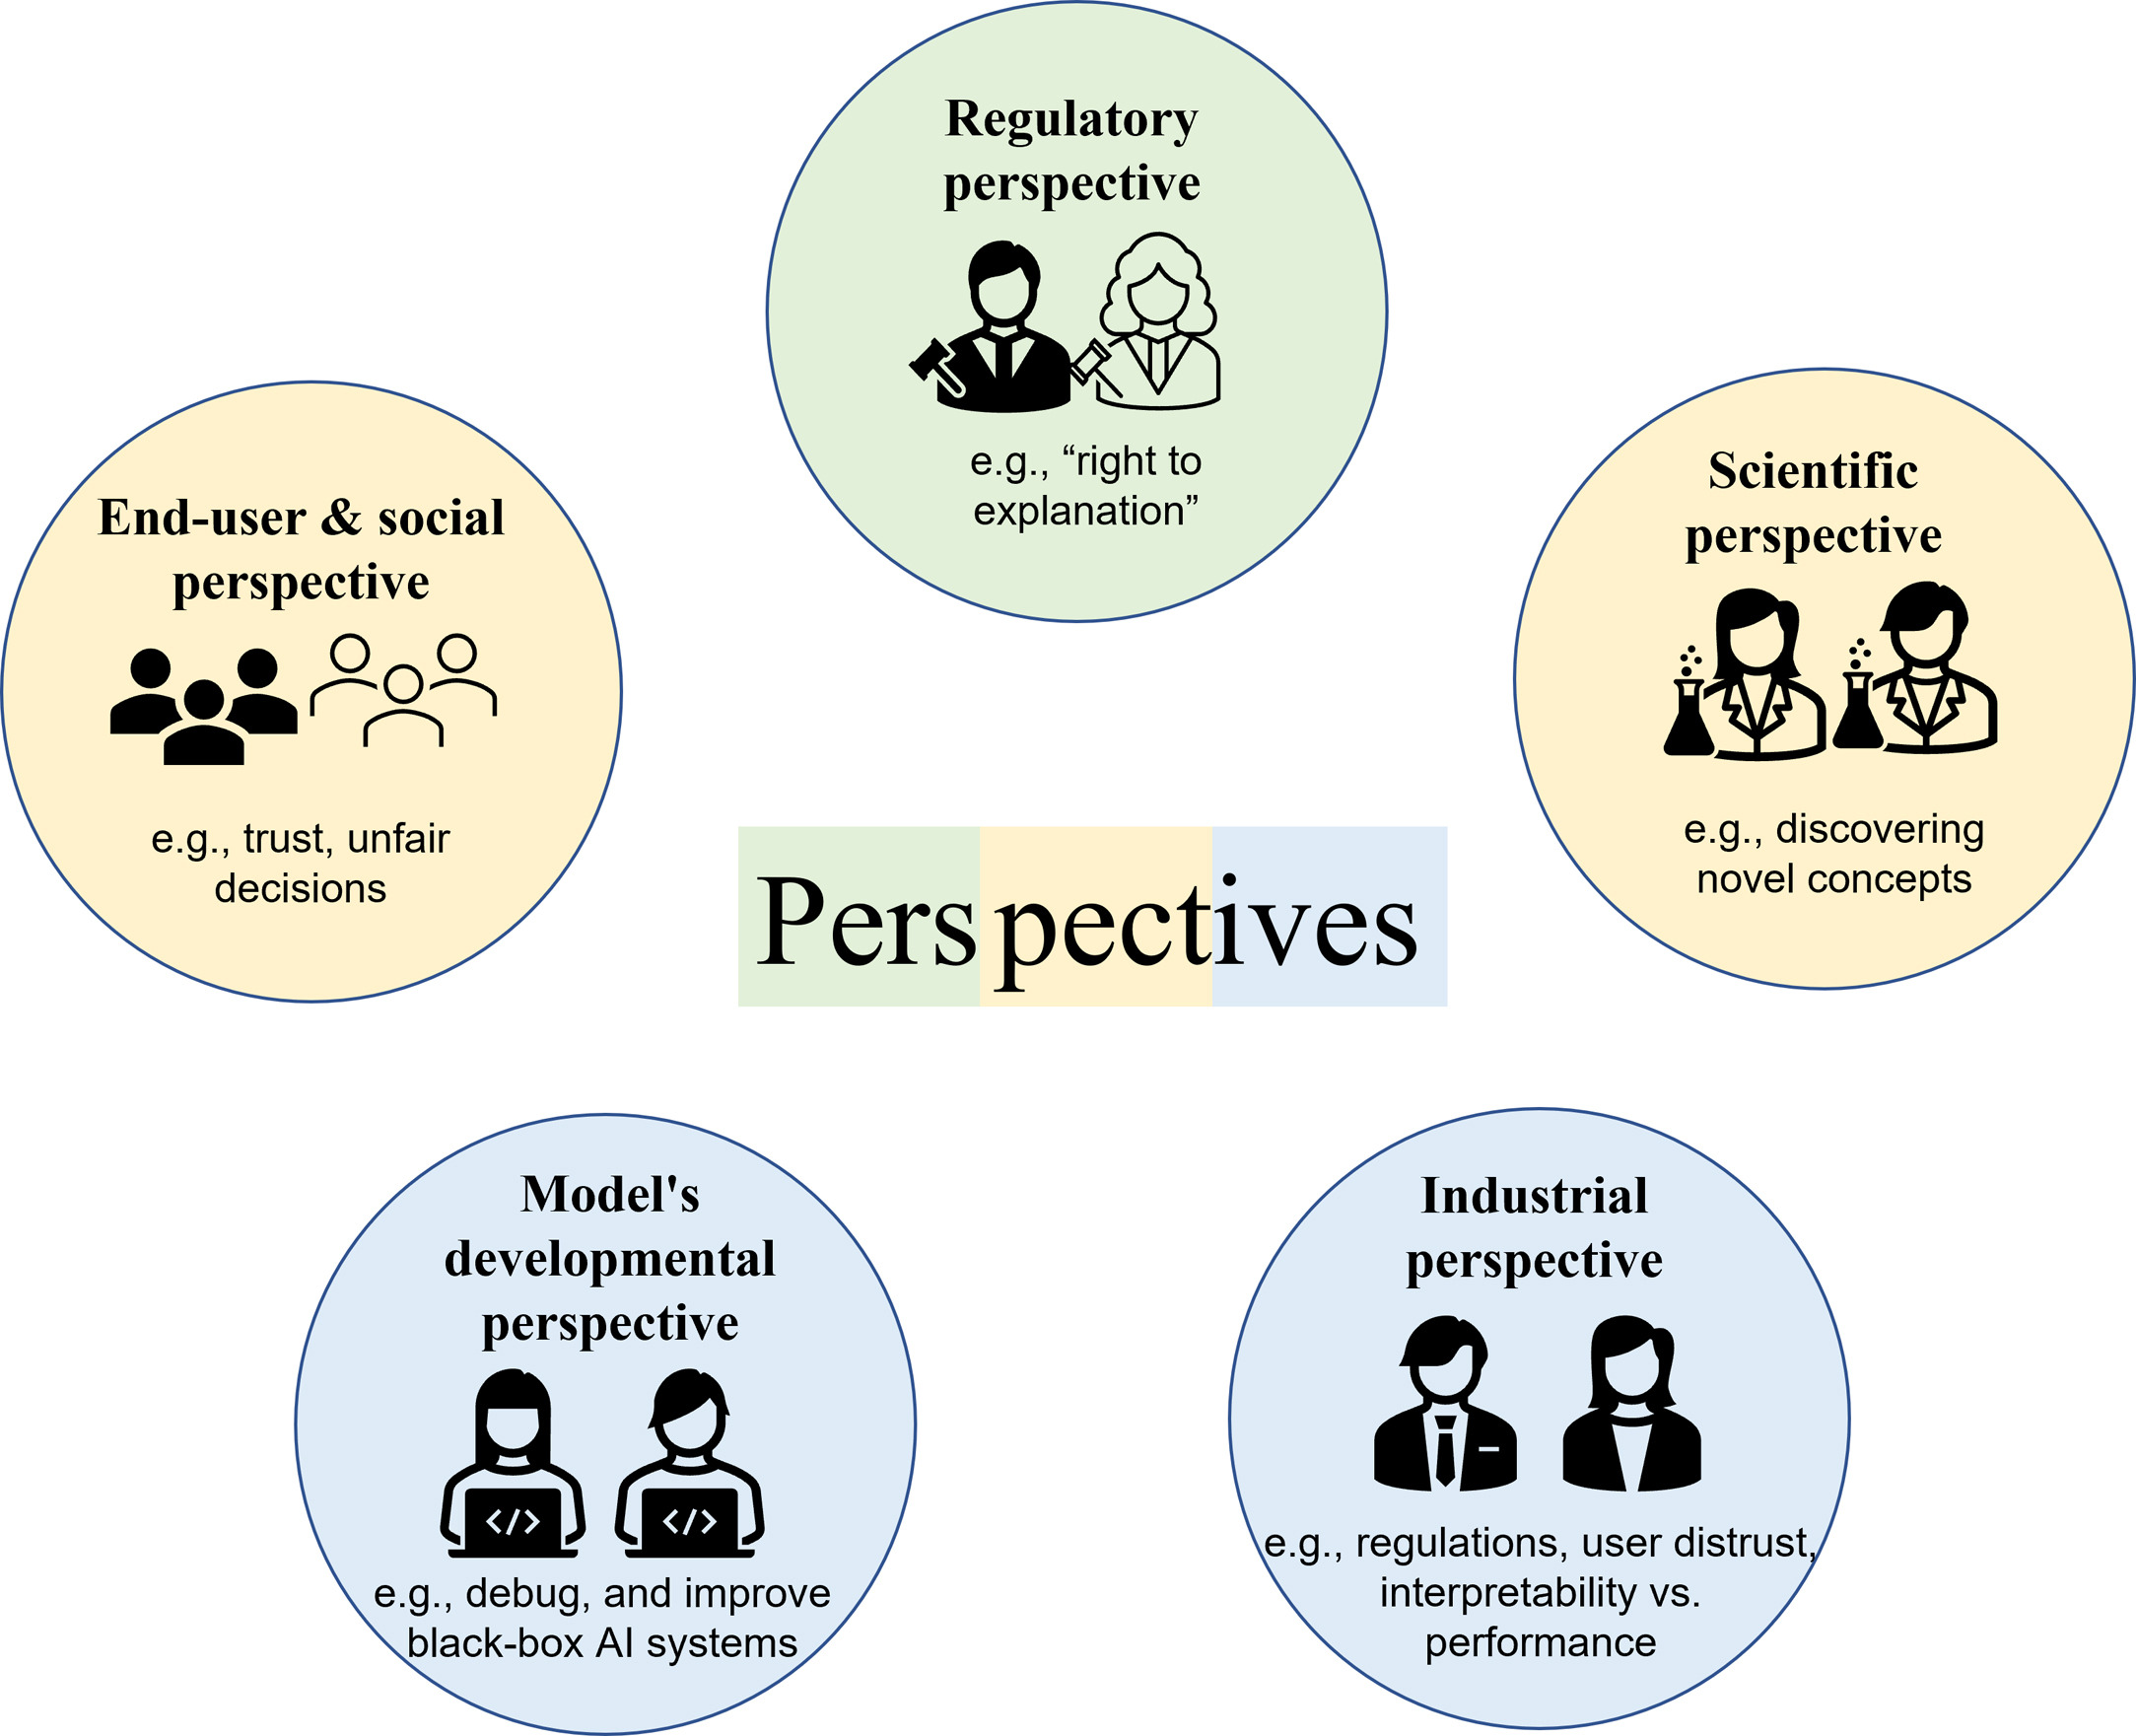
\includegraphics[width=0.5\textwidth]{img/motivation.jpg}
    \centering
    \caption{Summary of the main motivations regarding the use of XAI}
\end{figure}
We can summarize the motivation into 5 main points:
\begin{enumerate}
    \item Regulatory Perspective
    \item Scientific Perspective
    \item Industrial Perspective
    \item Model's developmental perspective
    \item End-user and social perspective
\end{enumerate}
\section{Motivation}
\subsection*{Regulatory Perspective}
Black-box AI systems are being utilized in many areas of our daily lives, which could be resulting in unacceptable decisions, especially those that may lead to legal effects. 
The European Union's General Data Protection Regulation (GDPR)\footnote{\url{https://www.privacy-regulation.eu/en/r71.htm}} is an example of why XAI is needed from a regulatory perspective. 
These regulations create what is called the \emph{right to explanation}, by which a user is entitled to request an explanation about the decision made by the algorithm that considerably influences them.

\subsection*{Scientific Perspective}
When building black-box AI models, we aim to develop an approximate function to address the given problem. 
Therefore, after creating the black-box AI model, the created model represents the basis of knowledge, rather than the data. 
Based on that, XAI can be helpful to reveal the scientific knowledge extracted by the black-box AI models, which could lead to discovering novel
concepts in various branches of science.

\subsection*{Industrial perspective}
Regulations and user distrust in black-box AI systems represent challenges to the industry in applying complex and accurate 
black-box AI systems. Less accurate models that are more interpretable may be preferred in the industry because of regulation
reasons. A major advantage of XAI is that it can help in mitigating the common trade-off between model interpretability and performance,
thus meeting these common challenges. 
However, it can increase development and deployment costs.

\subsection*{Model's developmental perspective}
Several reasons could contribute to inappropriate results for black-box AI systems, such as limited training data, biased training data, outliers, adversarial data, and model overfitting. 
Therefore, what black-box AI systems have learned and why they make decisions need to be understood, primarily when they affect humans lives. 
For that, the aim will be to use XAI to understand, debug, and improve the black-box AI system to enhance its robustness, increase safety and user trust, and minimize or prevent faulty behavior, bias, unfairness, and discrimination.

\subsection*{End-user and social perspective}
In the literature of deep learning, it has been shown that altering an image such that humans cannot observe the change can lead the model in producing a wrong class label (Adversarial Attacks). 
On the contrary, completely unrecognizable images to humans can be recognizable with high confidence using DL models.
Such findings could raise doubts about trusting such black-box AI models. 
The possibility to produce unfair decisions is another concern about black-box AI systems. 
This could happen in case black-box AI systems are developed using data that may exhibit human biases and prejudices.
Therefore, producing explanations and enhancing the interpretability of the black-box AI systems will help in increasing trust because it will be possible to understand the rationale behind the model's decisions, and we can know if
the system serves what it is designed for instead of what it was trained for. Furthermore, the demand for the fairness of black-box AI systems decisions, which cannot be ensured by error measures, often leads to the need for
interpretable models.

% \part{title}
\section{XAI - One topic, two keywords}
\begin{minipage}[c]{0.3\textwidth}
    \begin{figure}[H]
        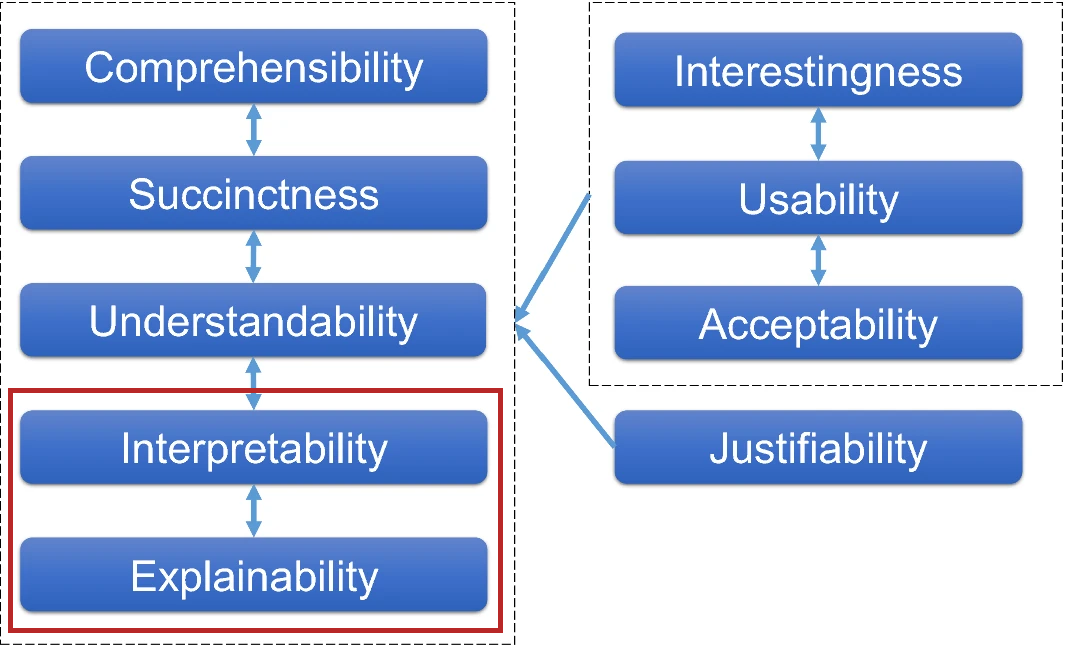
\includegraphics[width=\textwidth]{img/many_words.png}
        \centering
        \caption{Outline of the relationships between the common XAI terminologies}
    \end{figure}    
\end{minipage}
\hfill%
\begin{minipage}[c]{0.65\textwidth}
    In the Explainable AI domains there many terms that seems to be the same meaning.
    Specifically we are interested into two terms: Explainablility and Interpretability.\\
    
    Explainablility provide insights about an AI model while Interpretability tells if the insights make sense to the audience.
\end{minipage}

\section{Types of XAI}
\begin{minipage}[c]{0.5\textwidth}
    \begin{figure}[H]
        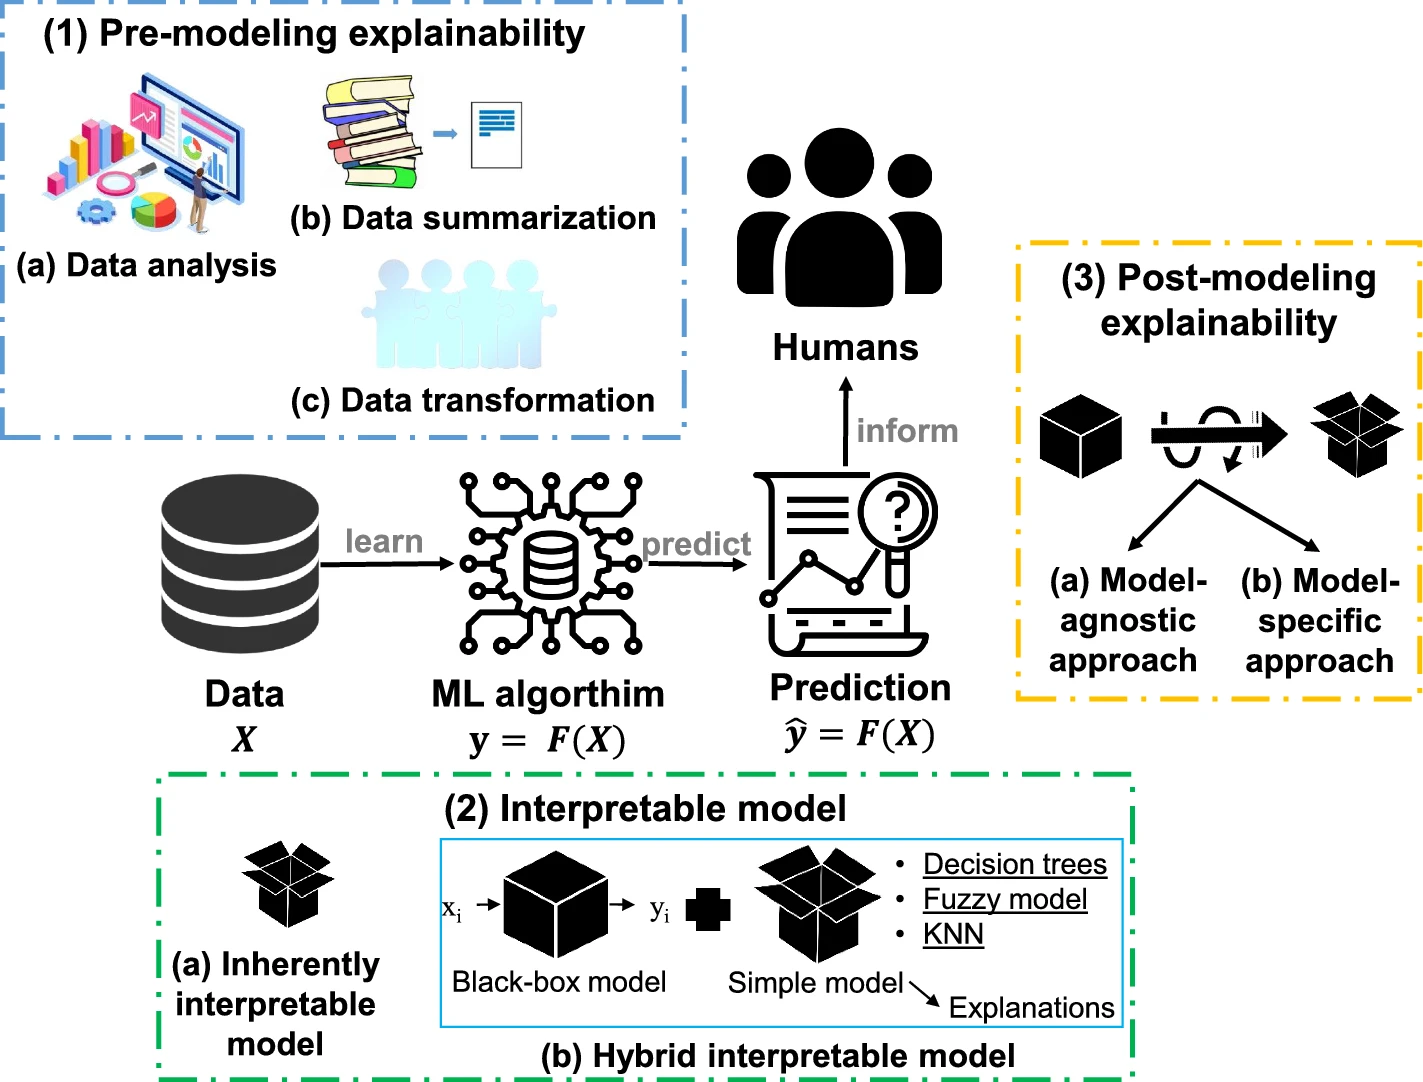
\includegraphics[width=0.8\textwidth]{img/types_XAI.png}
        \centering
        \caption{Outline of the relationships between the common XAI terminologies}
    \end{figure}
\end{minipage}
\begin{minipage}[c]{0.5\textwidth}
    There are three main types of Explainablility:
    \begin{enumerate}
        \item \textbf{Pre-modeling explainability}: summarize input data to identify most relevant features or aspects, based on statistical analysis. Some examples are: K-Means and PCA
        \item \textbf{Post-modeling explainability}: explain the results of a black-box model. Some tecniques include: 
        \begin{itemize}
            \item \emph{Feature relevance}: which input data mostly influences the output?
            \item \emph{Simplification}: aims to make a simplified version of the original model that has an
            optimized function, significantly reduces the complexity, has a simpler implementation
            process, and performance is comparable to the original version.
            \item \emph{Visualization}: interprets a models behavior by visual representations. Visualiza-
            tion techniques are considered the best way to explain the complicated inner interac-
            tions of the variables of the model, and they can be combined with other methods in
            order to increase their interpretability ability.
            \item \emph{Textual justifications}: explains a model by generating explanations in the form of
            text
            \item \emph{Contrastive explanations}: clarifies why an event occurred in contrast to another
        \end{itemize}
        \item \textbf{Interpretable models}: the model is not black-box on its own. some examples include: Linear or logistic regression and Decision trees
    \end{enumerate}
\end{minipage}\\

There are three main properties for interpretability:
\begin{itemize}
    \item Algorithmic transparency: The model can be expressed as a set of known mathematical or logical relations
    \item Decomposability: The model can be decomposed in submodules, with clear indication of connections between them
    \item Simulatability: The model can be easily simulated by a human, given only any input
\end{itemize}
\section{Causal analysis \& discovery}
Reconstructing the \textbf{causal relations} behind the phenomena we observe is 
a fundamental problem in all fields of science.
The traditional approach is to conduct active experiments, but in many fields
manipulations of the complex system under study are either impossible, 
unethical, or very expensive.
On the other hand, modern science generates an ever-growing amount of data 
from these systems, in particular time series data.
Concurrently, novel computing hardware today allows efficient processing 
of massive amounts of data. These developments have led to emerging interest 
in the problem of reconstructing causal networks or causal discovery from 
observational time series.\\

The definition of causality is that $X \rightarrow Y$ if and only if an intervention or
manipulation in $X$ has an effect on $Y$.
A practical example could be the altitude and the temperature as in Figure \ref{fig:tempvsheight}.
As the height increases the temperature lowers.

\begin{minipage}[c]{0.3\textwidth}
    \begin{figure}[H]
        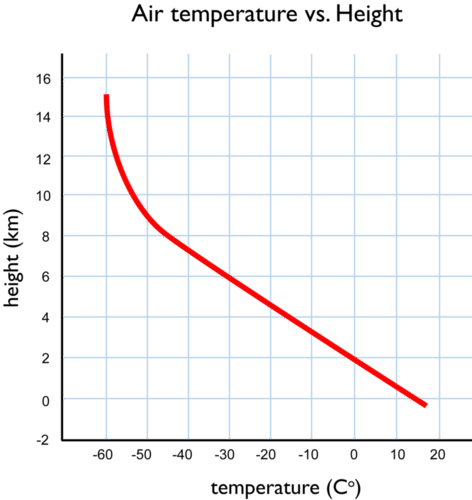
\includegraphics[width=0.6\textwidth]{img/tempvsheight.png}
        \centering
        \caption{Varion of temperature with respect to the height}
        \label{fig:tempvsheight}
    \end{figure}
\end{minipage}
\begin{minipage}[c]{0.6\textwidth}
    One of the main motivations behind causal analysis is a property called \textbf{similability}, 
    the ability o easily predict the output, given only any possible input.
\end{minipage}\\


We will consider causal analysis and discovery for time series since typically, 
input and output of a system are temporal signals, and we are interested in understanding 
how the system evolves and behaves over time.
This means, we want to understand how the temporal evolution of the output signal is affected
by the input signal (\textbf{and discovering which one is the input}).
We will denote as $V_T$ a variable $V$ which is observed for a temporal horizon $T$ (either continuous or
discrete)
\subsection{Structural causal model}
\begin{equation}
    V_t^j \coloneqq \textcolor{red}{f^j}(\textcolor{blue}{pa(V^j_t)}, \eta^j_t)\quad\text{for all }V_t^j\in \bm{V_t} \text{ and } t\in\mathbb{Z}
\end{equation}
Where $\textcolor{red}{f^j}$ is a generic non linear function, $\textcolor{blue}{pa(V^j_t)}$ are the parents of the variable $V^j$ i.e its causes and
$\eta^j_t$ is noise which comes from the uncertanty of the model or of the measurements.
\subsection{Granger's definition of causality (1969)}\label{sec:granger}
Given (temporal) variables $X$ and $Y$, we say that $X\;Granger-causes\;Y$
if $X$ contains information which affects $Y$ at time t, and such
information is not contained in the past of the universe ($Y$'s past or
other variables'past). In other words $Y$ depens \textbf{only} on $X$ and no other variables.If we only consider $Y$, we refer to bivariate causality \\

Granger's definition can be written in the following way as an autoregressive process:
\begin{equation}
    \bm{x_t}=\sum_{\tau=1}^{\tau_{max}}\phi(\tau)\bm{x}_{t-\tau}+\eta_t
\end{equation}
This formulation implies causality in mean (autoregressive model), this 
is a problem since it does not capture information about the distribution of the data.

\subsection{Conditional Mutual Information}
A more general definition comes from Schreibe: (bivariate) transfer entropy
\begin{equation}
    I^{TEbiv}_{X\rightarrow Y}=I(X_t^-;Y_t|Y_t^-)
    \label{eq:tebiv}
\end{equation}
where the `-` indicates the past of the variable and $I(X;Y|Z)$ denotes the Conditional Mutual Information (CMI).

\begin{equation}
    I(X;Y|Z)=\iiint{p(x,y,z)\log_2{\frac{p(x, y| z)}{p(x|z)\cdot p(y|z)}}dx\;dy\;dz}
    \label{eq:cmi}
\end{equation}
CMI (also called Related Entropy) comes from the concept of KL(Kullback-Leibler) divergence.
\begin{equation}
    D(p||q)=\sum_{x\in\mathcal{X}}p(x)\log{\frac{p(x)}{q(x)}}
\end{equation}
The KL divergence measures the degree of similarity (the distance) between two distribution namely $p$ and $q$.\\

The equation for the KL divergence seems to come out of the air, but in reality the equation is really simple...

We have two pieces, the first $\frac{p(x)}{q(x)}$ measures the distance between 
the distribution $p$ and the distribution $q$, then we add the $log$, we do that 
because if $p(x)=q(x)$ (i.e they are the same distribution) then the division will 
be 1. Since they are the same distribution the distance between the distributions should be 0 but for now it is only 1. 
If we add the $log$ then $\log(1)=0$ and so the distance is 0. The second piece $p(x)$ is a weight, this 
is used because we want to weight the distance based on the likelihood of the input
 $x$, this mean that we care less of high distance if the input is unlikely.
I've omitted a small detail, I've talked about distance between distributions 
but in reality what I meant was distance between points(e.g $p(x)$) in the 
distributions and so we need to add a summation to the equation 
(or an integral in case of continuous distributions) so to add the contribution
 of each individual point.\\

Similarly Mutual Information (MI) measures the \textbf{discrepancy} between \textbf{joint distribution} (p(x,y)) and the \textbf{product} (p(x)p(y)) of individual distributions.
Mutual Information(MI) is the same as CMI (eq \ref{eq:cmi}) but without the conditioning on $z$, so for the dicrete case the equation is:
\begin{equation}\label{eq:mi_disc}
    \begin{split}
        I(X;Y)&=\sum_{x\in\mathcal{X}}\sum_{y\in\mathcal{Y}}p(x,y)\cdot\log{\frac{p(x,y)}{p(x)p(y)}}\\
        &=D(p(x,y)||p(x)p(y))
    \end{split}
\end{equation}
This means that we can see MI as the KL divergence between the joint distribution and the product distribution.

\begin{tcolorbox}[colbacktitle=black!7!white,coltitle=black!75!white,title=\textbf{Statistics Recall}]
Let's make a quick statistics recall:\\
Given two random variables $x$ and $y$ if $x \text{ \textbf{indipendent}of } y$\\
$p(x,y) = p(x)p(y)$ so the product distribution is equal to the joint distribution\\\\
Given two random variables $x$ and $y$ if $x \text{ \textbf{dependent }on } y$\\
$p(x,y)=p(y)\cdot p(x|y)$
\end{tcolorbox}

So with MI we are trying to check if $x$ and $y$ are dependent:\\

\begin{center}
    \begin{minipage}[t]{0.4\textwidth}
        \noindent
        Assume $x$ and $y$ are \textit{\textbf{independent}}:
        \begin{equation}
            \begin{split}
                I(X;Y)&=\sum_{x\in\mathcal{X}}\sum_{y\in\mathcal{Y}}p(x,y)\cdot\log{\frac{\textcolor{red}{p(x,y)}}{p(x)p(y)}}\\
                &=\sum_{x\in\mathcal{X}}\sum_{y\in\mathcal{Y}}p(x,y)\cdot\log{\frac{\textcolor{red}{p(x)p(y)}}{p(x)p(y)}}\\
                &=\sum_{x\in\mathcal{X}}\sum_{y\in\mathcal{Y}}p(x,y)\cdot\log{\cancel{\frac{p(x)p(y)}{p(x)p(y)}}}\\
                &=\sum_{x\in\mathcal{X}}\sum_{y\in\mathcal{Y}}p(x,y)\cdot\log{1}\\
                &=\sum_{x\in\mathcal{X}}\sum_{y\in\mathcal{Y}}p(x,y)\cdot0\\
                &=0
            \end{split}
        \end{equation}
    \end{minipage}
    \begin{minipage}[t]{0.4\textwidth}
        \noindent
        Assume $x$ and $y$ are \textit{\textbf{dependent}}:
        \begin{equation}
            \begin{split}
                I(X;Y)&=\sum_{x\in\mathcal{X}}\sum_{y\in\mathcal{Y}}p(x,y)\cdot\log{\frac{\textcolor{red}{p(x,y)}}{p(x)p(y)}}\\
                &=\sum_{x\in\mathcal{X}}\sum_{y\in\mathcal{Y}}p(x,y)\cdot\log{\frac{\textcolor{red}{p(y)p(x|y)}}{p(x)p(y)}}\\
                &=\sum_{x\in\mathcal{X}}\sum_{y\in\mathcal{Y}}p(x,y)\cdot\log{\frac{\cancel{p(y)}p(x|y)}{p(x)\cancel{p(y)}}}\\
                &=\sum_{x\in\mathcal{X}}\sum_{y\in\mathcal{Y}}p(x,y)\cdot\log{\frac{p(x|y)}{p(x)}}\\
                &\ne 0
            \end{split}
        \end{equation}
    \end{minipage}
\end{center}
% \newpage
So to recap:
\begin{itemize}
    \item $x \text{ and } y$ DEPENDANT$\rightarrow\;MI\ne 0$
    \item $x \text{ and } y$ INDIPENDENT$\rightarrow\;MI=0$
\end{itemize}
CMI(Eq \ref{eq:cmi}) is essentially the same but we measure if two variables are dependent given that both are conditioned by a third variable.
In other words given $x,y \text{ and } z$ how much $x$ and $y$ are indipendent given that both depend on $z$.
Differently from Granger Causality (Section \ref{sec:granger}) in MI and CMI 
we are evaluating the entire distribution instead of only the mean so it is 
more informative.\\
Given the above definition we can generalize the Granger formulation to include CMI:\\
$I^{FullCI}_{i\rightarrow j}(\tau)=I(X^i_{t-\tau};X^j_t|\bm{X}_t^{(t-1,\ldots,t-\tau_{max})}\setminus\{X^i_{t-\tau}\})$ 
\\here $\bm{X}_t^{(t-1,\ldots,t-\tau_{max})}$ is what we called $Z$ before i.e the past of all the variables.\\

To better understand causasality we can visualize it as a graph:
\begin{figure}[H] \label{fig:causalgraph}
    \centering
    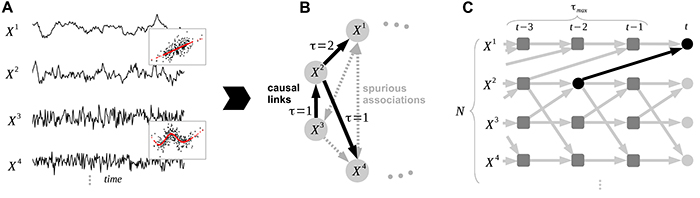
\includegraphics[width=0.8\textwidth]{img/visualization.jpeg}
    \caption{A time series dataset (panel A) from a complex system of which we try to reconstruct the underlying causal dependencies (panel B), 
    accounting for linear and nonlinear dependencies and including their time lags (link labels). }
\end{figure}
Figure \ref{fig:causalgraph}B represents the causal realation between variables, you can see solid and dashed lines.
The first represents a real causal relation between variables, while the second represent what's called a spurious association, 
this means that we find a relation between variables but those varibles are not related and this relation occurs either by chance 
or it is caused by a third unseed variable.\\\\
A simple example of this can be a causal graph representing the relation between the \emph{number of ice cream cones sold} in a city
per month and the \emph{number of sunburn cases} reported in the city per month.
If we analize that graph we can see that the number of ice cream cones sold in one month causes the number of sunburn cases reported in the next month.
Intuitively this relation does not make sense, how is it possible that an increase in number of ice creams sold causes the number of sunburs to raise?
In fact this relation is spurious since both are caused by a third variable, namely the \emph{average temperature} in the city per month.
Higher temperatures cause more people to buy ice cream and also expose themselves to the sun, leading to more sunburns.
As you can see in the picture on top of the edges there is written a number, it states the time lag difference in the relation, to make it more clear 
let's go back to the ice cream example. Assume $X^3$ is the number of ice cream sold and $X^2$ represents the number of sun burns.
As we said before the number of ice cream cones sold in one month causes the number of sunburn cases reported in the \textbf{next month}, 
here the key point is next month, as we can see in the graph is written as $\tau=1$ this means that $X^3_{t-1}\rightarrow X^2_{t}$, where the arrow represents the causal realtion.

% TODO: Figure \ref{fig:causalgraph}C

\subsection{Causal Discovery}
The goal of causal discovery is to identify causal links, distinguishing them from spurious associations depending on inherent
correlations between variables.
Before doing so we may need to make some assumptions on the nature of time series variables
(i.e., on the underlying system's structure).

\subsubsection*{Causal sufficiency}
\begin{tcolorbox}[colback=red!5!white,colframe=red!75!black,title=\textbf{Causal sufficiency Definition}]
    A set $W\subset V\times\mathbb{Z}$ of variables is causally sufficent for a process \textbf{X} if and only if in the process 
    every common cause of any two or more variables in $W$ is in $W$ or has the same values for all units in the population.
\end{tcolorbox}
This simply means that it is never the case that a variable is determined on all other variables at all possible delays.\\
\begin{figure}[H]
    \centering
    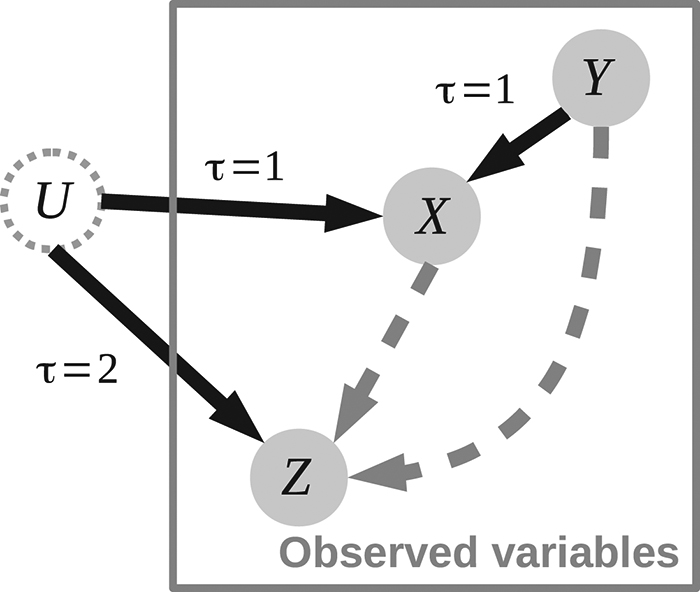
\includegraphics[width=0.2\textwidth]{img/causalsuff.jpeg}
    \caption{Example where Cusal Sufficency does not hold}
    \label{fig:causalsuff}
\end{figure}
Causal Sufficency is not always true, as we can see in Figure \ref{fig:causalsuff}, there if we dont't
observe the spurious variable $U$ we have that $Z$ depends on all the varibles (namely $X$ and $Y$).

\subsubsection*{Causal Markov Condition}
\begin{tcolorbox}[colback=red!5!white,colframe=red!75!black,title=\textbf{Separation Definition}]
    Two nodes $A$ and $B$ are separated given a conditioning set $S \text{ with } A, B \notin S$ 
    ($S$ may also be empty) if all paths between $A$ and $B$ are blocked, denoted:
    $A\bowtie B|S$.
\end{tcolorbox}
This simply means that a path is blocked if no link is available between two variables.
An example can be found in Figure \ref{fig:causalgraph}C where $X^1_t$ and $X^4_{t-1}$ have the path blocked.
\begin{tcolorbox}[colback=red!5!white,colframe=red!75!black,title=\textbf{Cusal Markov condition Definition}]
    The joint distribution of a time series process $\bm{X}$ with
    graph $G$ fulfills the Causal Markov Condition if and only if
    for all $Y_t\in \bm{X}_t$ with parents $\mathcal{P}_{Y_t}$ in the graph\\
    \begin{equation*}
        \bm{X}^-_t\setminus\mathcal{P}_{Y_t}\bowtie Y_t | \mathcal{P}_{Y_t}\implies\bm{X}^-_t\setminus\mathcal{P}_{Y_t}\Perp Y_t | \mathcal{P}_{Y_t}
    \end{equation*}
    that is, from separation in the graph (since the parents $\mathcal{P}_{Y_t}$ separate$Y_t$ from $\bm{X}^-_t\setminus\mathcal{P}_{Y_t}$ in the graph) follows indipendence.
\end{tcolorbox}
This definition simply means that if there is no path between two variables those are indipendent (indicated with the symbol $\Perp$) or said differently if we know $\mathcal{P}_{Y_t}$ (parents of $Y_t$) no other variable influences $Y_t$.
From this definition easily follows that Separation implies indipendence.

\subsubsection*{Faithfulness}
\begin{tcolorbox}[colback=red!5!white,colframe=red!75!black,title=\textbf{Faithfulness Definition}]
    The joint distribution of a time series process $\bm{X}$ with
    graph $G$ fulfills the Faithfulness condition if and only if for all
    disjoint subsets of nodes (or single nodes) $A, B, S \subset\mathcal{G}$ it
    holds that
    \begin{equation*}
        X_a \Perp X_b|X_S\implies A\bowtie B|S
    \end{equation*}
    that is, from independence follows separation, which includes its logical contraposition
    \begin{equation*}
        A\cancel{\bowtie} B|S\implies X_a \cancel{\Perp} X_b|X_S
    \end{equation*}
    from connectedness follows dependence.
\end{tcolorbox}
This definition states that from Indipendence follows Separation.

Intuitively, Faithfulness together with the Causal Markov Condition 
allow us to conclude that a measured
statistical dependency is actually due to some causal mechanism and, conversely,
a measured independence implies that no direct causal mechanism exists.
Both conditions are an important assumption for causal discovery algorithms that we'll discuss later.

\subsubsection*{Causal Stationarity}
\begin{tcolorbox}[colback=red!5!white,colframe=red!75!black,title=\textbf{Definition}]
    The time series process $\bm{X}$ with graph defined in \ref{fig:causalgraph}C is called causally stationary 
    over a time index set $\mathcal{T}$ if and only if for all links $X^i_{t-\tau}\rightarrow X^j_\tau$ in the graph
    \begin{equation*}
        X^i_{t-\tau}\cancel{\Perp}X^j_\tau|\bm{X}^-\setminus\{X^i_{t-\tau}\}\text{ holds for all } t\in\mathcal{T}
    \end{equation*}
\end{tcolorbox}
This constitutes actually a weaker form of stationarity than the common definition of stationarity in mean, 
variance, spectral properties, or of the value of individual coefficients in a linear model.
Intuitively this definition states that if I find a causal relation this should be time indipendent.\\

A typical reason for non-stationarity are confounder variables, i.e., wrong assumption in causal sufficiency.

\subsubsection*{Dependency (functional) type}
To test conditional independence hypotheses $X \Perp Y \;|\; Z$ different test statistics can be utilized.
These are typically based on making certain assumptions about the type of the underlying dependency structure.
While classical statistical methods are often based on the assumption of linearity (which
allows us to derive rigorous results), modern statistics, the physics community, and the recent 
field of machine learn-ing have developed non-parametric or model-free methods that allow us to better 
capture the nonlinear reality of many dynamical complex systems—at the cost of weaker theoretical results.
Conditional independence testing can be classified into regression-based and model-free approaches.\\
\begin{itemize}
    \item \textbf{Regression Based}: Regression-based conditional independence tests of $X\Perp Y\;|\;Z$ are based on 
    first regressing out the influence of Z from X and Y and then testing the dependence between the residuals.\\
    We first fit a model assuming:
    \begin{eqnarray*}
        X=f_X(Z)+\epsilon_X\\
        Y=f_Y(Z)+\epsilon_Y
    \end{eqnarray*}
    for centered variables $X, Y$ and independent and identicallynormally distributed $\epsilon_{X,Y}$.
    Secondly, from the estimated functions $\hat{f}$, the residuals are formed as
    \begin{eqnarray*}
        r_X=X-\hat{f}_X(Z)\\
        r_Y=Y-\hat{f}_Y(Z)
    \end{eqnarray*}
    Finally, the dependence between the residuals can be tested with different pairwise association tests (e.g., t-test).\\
    \item{\textbf{Model Free}}: model-free methods directly test conditional independence.
\end{itemize}

\begin{figure}[H]
    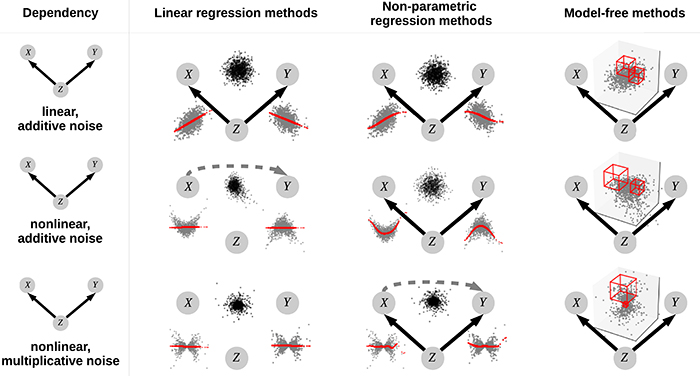
\includegraphics[width=0.9\textwidth]{img/depfunc.jpeg}
    \centering
    \caption{Illustration of applicability of different conditional independence methods(linear and non-parametric
    regression-based and model-free) on different types of linear and nonlinear common driver models. Black arrows 
    denote correctly identified causal links and dashed gray arrows indicate spurious links. The gray scatterplots 
    with red fit line illustrate regressions of X and Y on Z and the black scatterplot the dependency between the 
    residuals $r_X,r_Y$. The three-dimensional scatterplot with red cubes in the right column depicts the CMIknn test 
    which is based on data-adaptive nearest-neighbor estimation (the cubes are smaller for denser regions).}
\end{figure}

Model-free regression generally works, but they are very data-hungry and computationally expensive.

\subsection{Causal Discovery Algorithms}
\begin{tcolorbox}[colback=red!5!white,colframe=red!75!black,title=\textbf{Universal causal consistency Definition}]
Denoted by $\mathcal{\hat{G}}_n$ the estimated graph of some causal estimator from a sample of a 
distribution $P$ with sample size $n$ and by $\mathcal{G}$ the true causal graph. 
Then a causal estimator is said to be universally consistent if $\hat{\mathcal{G}}_n$ 
converges in probability to $\mathcal{G}$ for every distribution $P$,
\begin{equation*}
    \lim_{n\rightarrow\infty} Pr(\hat{\mathcal{G}}_n\ne\mathcal{G})=0
\end{equation*}
\end{tcolorbox}
Consistency is an important property of causal methods that tells us whether the method provably 
converges to the true causal graph in the limit of infinite sample size. That is, the probability of estimating 
the wrong graph becomes arbitrarily small if enough data is available, for any distribution $P$ (hence “universal”).

\subsubsection{FullCI Algorithm}
This is the simples algorithm that one can come up with, it tests for conditional independence between each
$X^i_{t-\tau}$ and $X^j_t$ conditioned on the entire past $\bm{X}_t^{(t-1,\;\ldots\;, t-\tau_{max})}$ excluding $X^i_{t-\tau}$.
\begin{equation}
    I^{FullCI}_{i\rightarrow j}(\tau)=I(X^i_{t-\tau};X_t^j|\bm{X}_t^{(t-1,\;\ldots\;, t-\tau_{max})}\setminus\{X^i_{t-\tau}\})
\end{equation}
This approach strongly suffers from the curse of dimensionality.
Complexity depends on the functional dependency assumption, assuming Linear dependency the complexity is
$\mathcal{O}(n(N\tau_{max})^2)$, where $N$ is the number of variables and $n$ is the sample size.

\subsection{Optimal Causation Entropy (OCE)}
A discovery algorithm based on the information-theoretic optimal causation entropy principle which reconstructs 
the lagged parents of a variable $X_t^j$ by an \textbf{iterative} procedure alleviating the curse of dimensionality.
Evaluates CMI \& Mutual Information (MI) in a forward-backward scheme for each variable.

\begin{equation}
    I(X;Y)=\int_Y\int_X{p(x,y)\log_2{\frac{p(x, y)}{p_1(x)p_2(y)}}dx\;dy}
\end{equation}
\begin{itemize}
    \item Forward: populate causal parents $\mathcal{P}^{OCE}(X^j_t)=\emptyset$
        \begin{itemize}
            \item 1st parent $\leftarrow$ maximize $I(X^i_{t-\tau};X^j_{t})$ for all $X^i_{t-\tau}\in\bm{X}_t^-$
            \item 2nd parent $\leftarrow$ maximize CMI $I(X^i_{t-\tau};X^j_{t}|X^{(1)})$
            \item 3rd parent $\leftarrow$ maximize CMI $I(X^i_{t-\tau};X^j_{t}|X^{(1)},X^{(2)})$
            \item $\ldots$ until CMI is significant (e.g., with t-test or non-linear methods) at each step we condition on all previous parents
        \end{itemize}
    \item Backward: prune not significant parents
    \begin{equation*}
        X^i_{t-\tau}\Perp X^j_{t} \;|\; \hat{\mathcal{P}}^{OCE}(X^j_t)\setminus\{X^i_{t-\tau}\}\quad
        \forall X^i_{t-\tau}\in\hat{\mathcal{P}}^{OCE}(X^j_t)
    \end{equation*}
    This means if the variable ($X^j_{t}$) is conditionally indipendent of a parent ($X^i_{t-\tau}$) given all the other parents
    excluded the parent we are evaluating ($\hat{\mathcal{P}}^{OCE}(X^j_t)\setminus\{X^i_{t-\tau}\}$) we can remove $X^i_{t-\tau}$
\end{itemize}

This algorithm has two main \textbf{\textcolor{Green}{advantages}}:
\begin{itemize}
    \item It is not necessary to condition on all variables and on all times
    \item The complexity is polynomial
\end{itemize}
While the main \textbf{\textcolor{Red}{drawback}} is that useless parents are added.
\section{Application of causal discovery to a real system}
\begin{figure}[H]
    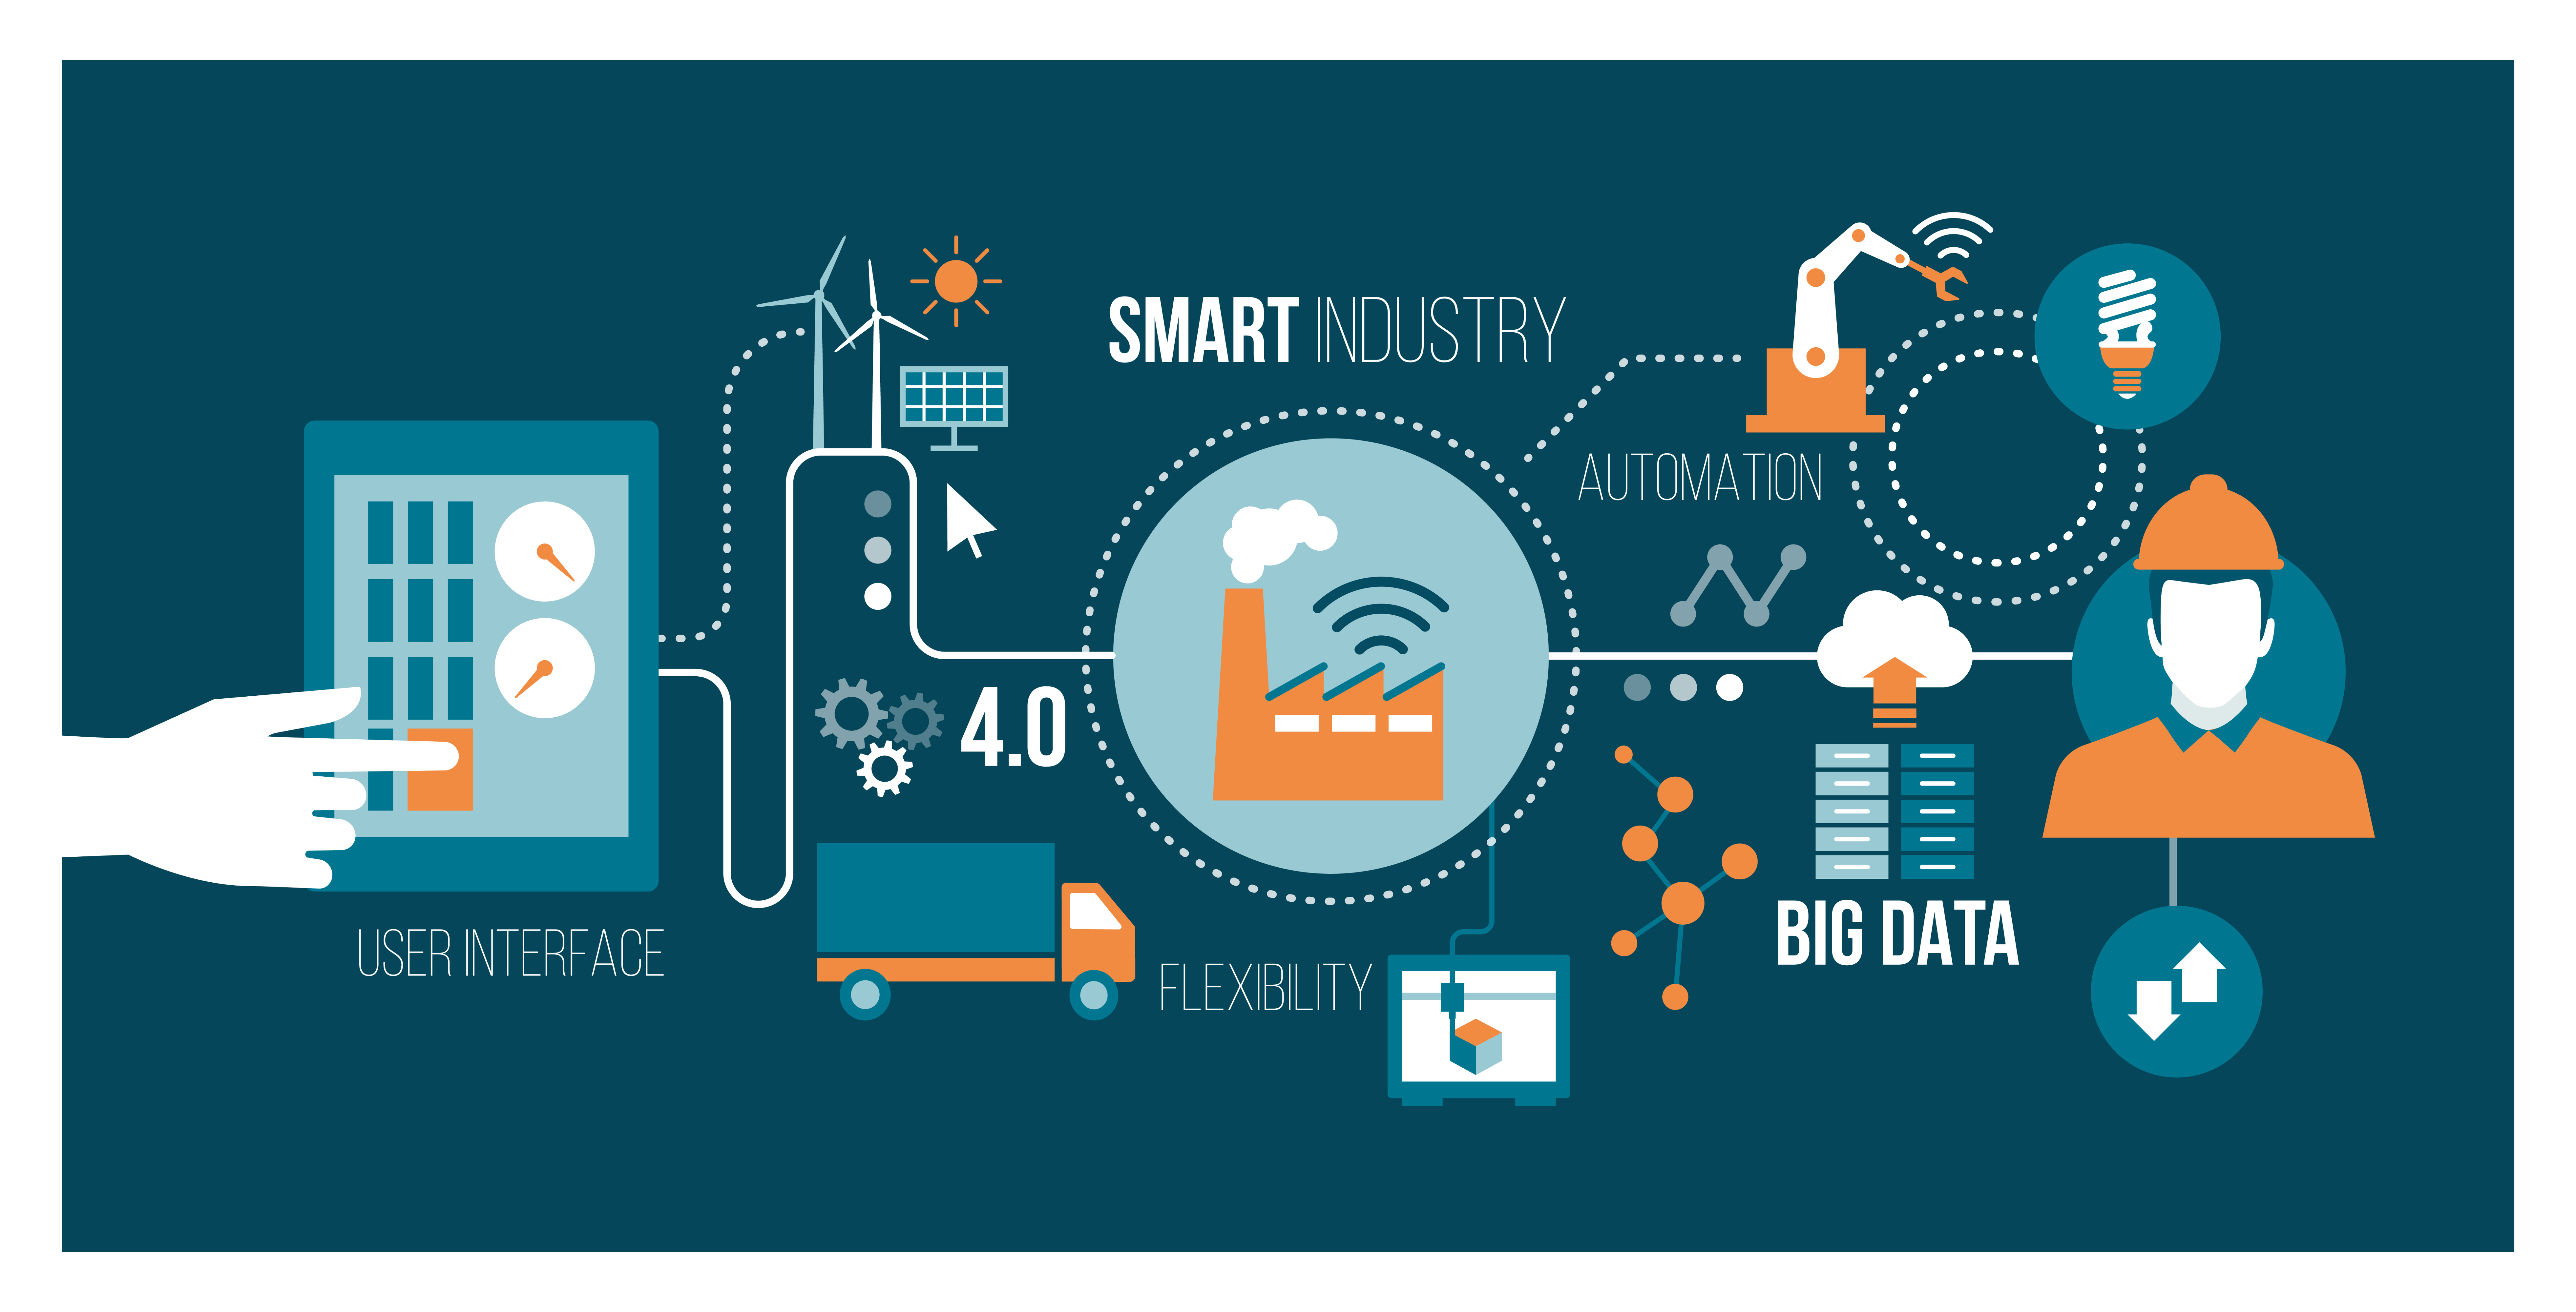
\includegraphics[width=0.7\textwidth]{img/industry4.jpg}
    \centering
    % \caption{'caption'}
\end{figure}
\subsection{Cyber-physical systems(CPS)}
Cyber-physical systems are characterized by a tight interaction between
computational units and physical environment. Those systems have high interaction with humans.
Robots, Industrial Control Systems, Smart Grids and Buildings, Autonomous Cars, $\ldots$ are some examples of CPS.

Those systems pose some Risks (and Challenges) like:
\begin{itemize}
    \item Safety of operators
    \item Cyber attacks
    \item Continual operation
    \item Errors and anomalies are very difficult to detect, due to
    complex physics, architecture and connection of the system.
\end{itemize}

XAI has a great potential for human-machine interaction, predictive maintainance and anomaly
detection, leading to a better exploitation of CPS.

An example of CPS is the SWaT (Secure Water Treatment), a small realistic replication (90
sqm) of a real plant for water filtration and dechlorination in big cities.
It contains 51 sensors/actuators, the dataset contains 11 days of operation.
This example is a well known benchmark for for CPS study and analysis, 
cyber security and assessment of anomaly detection algorithms.
\begin{minipage}[t]{0.4\textwidth}
    \begin{figure}[H]
        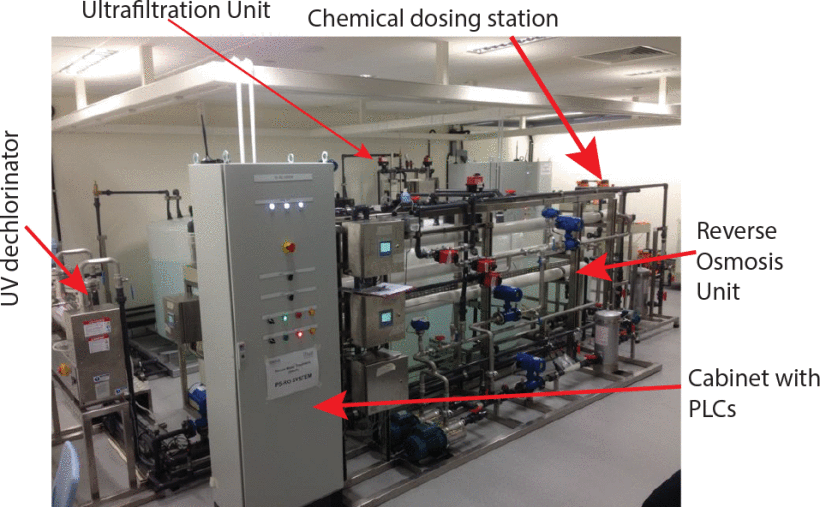
\includegraphics[width=\textwidth]{img/swat.png}
        \centering
    \end{figure}
\end{minipage}
\begin{minipage}[t]{0.5\textwidth}
    \begin{figure}[H]
        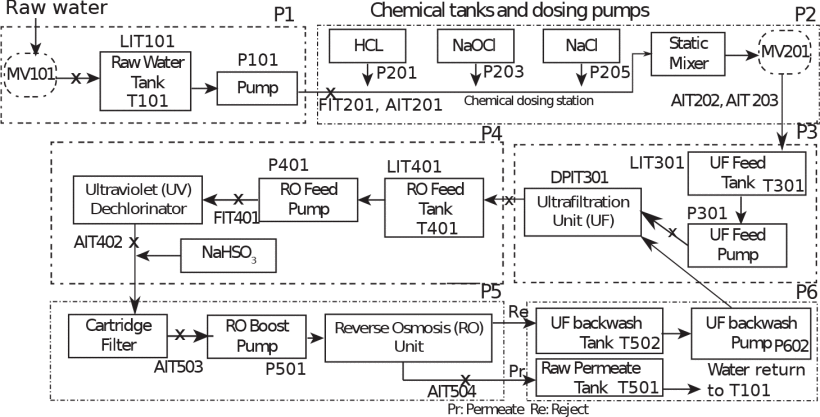
\includegraphics[width=\textwidth]{img/swat_schema.png}
        \centering
    \end{figure}    
\end{minipage}

\subsection{Anomaly Detection}
Physical Systems must ensure continuous operation to do so there is the field of 
Anomaly Detection which goal is to detect anomalies by observing time series representing a system.
There are various approaches:
\begin{itemize}
    \item Online vs Offline
    \item Supervised vs Unsupervised
    \item Single Class vs Open Class
\end{itemize}

\subsubsection*{Unsupervised single class anomaly detection}
\textbf{Online pipeline}
    \begin{itemize}
        \item Collect a dataset of normal behavior
        \item Train a normal model
        \item Use normal model as predictor on anomalous model
        \item Verify discrepancy between prediction and actual readings
    \end{itemize}
Some Algorithms include:
\begin{itemize}
    \item Regression
    \item SVM
    \item PCA
    \item Neural networks
\end{itemize}

\textbf{Offline pipeline}
\begin{itemize}
    \item Collect a dataset of normal behavior
    \item Train a normal model
    \item Train an anomalous model and check the difference with the normal one (or train a model on normal and anomalous data to classify them).
\end{itemize}
\subsubsection*{The role of causal analysis}
Offline anomaly detection identifies normal and anomalous instances of the CPS process, but they don't tell:
\begin{itemize}
    \item What's the origin of the anomaly?
    \item How do multiple anomalies differ?
\end{itemize}
Causal analysis can explain the anomaly.

\section{Explainable models of agency}
This section deals with the application of XAI to Autonomous Agents (and Autonomous Planning).
\subsection{What is an agent?}
An agent is anything that can be viewed as perceiving its environment through sensors and
acting upon that environment through actuators. A human agent has eyes, ears, and other organs for sensors and hands, legs, vocal tract,
and so on for actuators. A robotic agent might have cameras and infrared range finders for
sensors and various motors for actuators.
We use the term percept to refer to the content an agent's sensors are perceiving. An
agent's percept sequence is the complete history of everything the agent has ever perceived.\\

We use the term percept to refer to the content an agent's sensors are perceiving. An
agent's percept sequence is the complete history of everything the agent has ever perceived.
Mathematically speaking, we say that an agent's behavior is described by the agent function that maps any given
percept sequence to an action.

\begin{center}
    \begin{minipage}[t]{0.3\textwidth}
        \begin{figure}[H]
            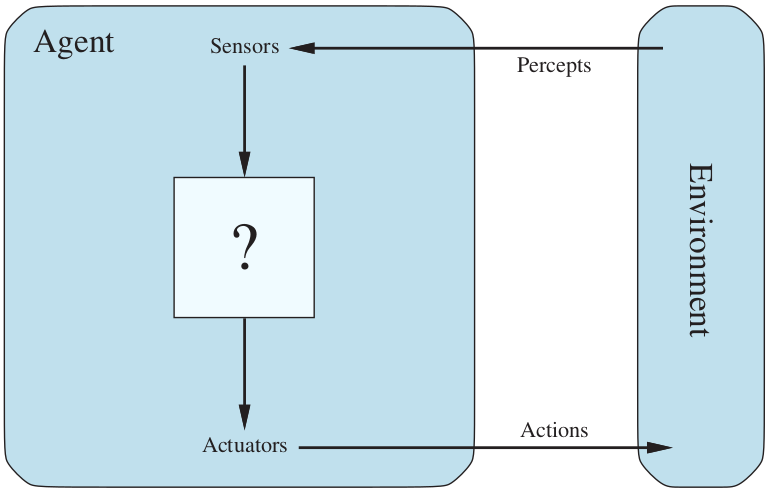
\includegraphics[width=\textwidth]{img/agent.png}
        \end{figure}
    \end{minipage}
    \hspace{2cm}
    \begin{minipage}[t]{0.4\textwidth}
        \begin{figure}[H]
            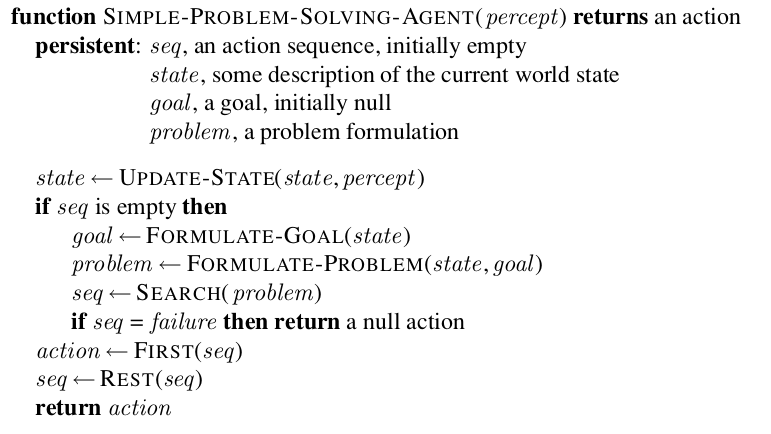
\includegraphics[width=\textwidth]{img/simpleprobsolving.png}
        \end{figure}
    \end{minipage}
\end{center}

A simple example of an autonomous agent and an environment is a robot playing chess.

How does humans play chess? 
\begin{itemize}
    \item We know the rules
    \item We observe the current state of the environment
    \item We \textbf{reason on the rules and the state}, and \textbf{infer} the next action (or even plan a short-term sequence)
\end{itemize}

This process of reason on the rules and the state is called Deductive Reasoning.
The definition of Deductive Reasoning is to infer facts from known other facts and rules.

\subsection{Logic}
A logic formalism is defined in terms of:
\begin{itemize}
    \item \textbf{Syntax}: symbols
    \item \textbf{Semantics}: the meaning of symbols
\end{itemize}
Formulas (or sentences) may be true or false depending on the value of variables
\begin{itemize}
    \item Sentence: $x+y=2$
    \item Model 1: $\{x=1,y=1\}\rightarrow$ sentence is true
    \item Model 2: $\{x=1,y=0\}\rightarrow$ sentence is false
\end{itemize}
A model $M$ is a possible assignment of all variables in a domain $D$.

The model of a formula $f$ in $D$, i.e., $M(f)$, is the set of assignments where $f$ holds.

\subsection{Propositional Logic}
\begin{figure}[H]
    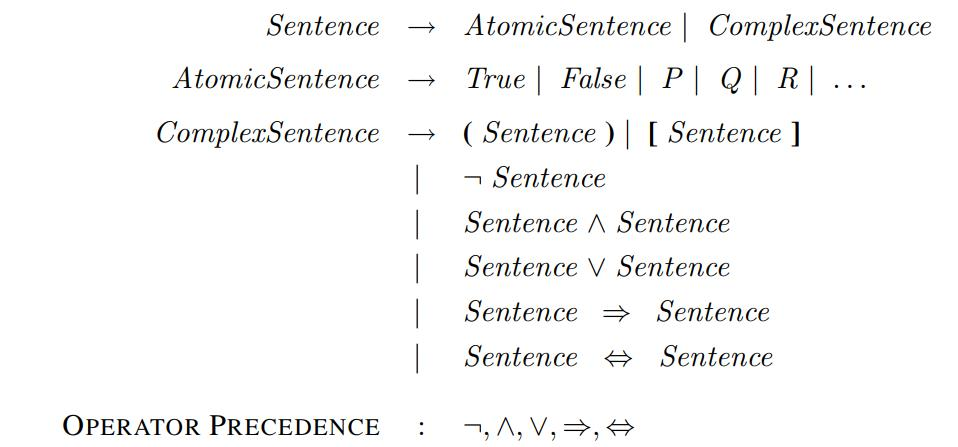
\includegraphics[width=0.7\textwidth]{img/proplogic.png}
    \centering
\end{figure}

\subsection{Logic Inference}

\begin{eqnarray*}
    \alpha \models \beta \text{ if and only if } M(\alpha)\subseteq M(\beta)\\
    \text{where } \alpha \text{ and } \beta \text{ are two formulas, } \\
    M(\alpha) \text{ and } M(\beta) \text{ are models (i.e assignments)}
\end{eqnarray*}

The $\models$ symbol is called entails. An example of entailment is $\alpha=\land,\; \beta=\lor$.

\begin{table}[H]
    \centering
    \begin{tabular}{lllll}
    \multicolumn{2}{c}{{\textbf{Variables}}} &  & \multicolumn{2}{l}{\textbf{Logical Operators}} \\
    $X_1$ & $X_2$ &  & $\land$ & $\lor$ \\
    0        & 0       &  & 0       & 0      \\
    0        & 1       &  & 0       & 1      \\
    1        & 0       &  & 0       & 1      \\
    1        & 1       &  & 1       & 1     
    \end{tabular}
\end{table}
As we can see from the table above the set of values of $X_1$ 
and $X_2$ where $\lor$ is True is a superset of the set of values 
where $\land$ is True.
Said in another way $\land\models\lor$ since $M(\land)\subset M(\lor)$.

The scope of Logical Inference is to entail formulas from a set of fomulas named Knowledge Base (KB). \\
$KB\models \gamma$.
Some desirable properties are Soundness(i.e No false positives) and Completeness (i.e the ability to entail all possible formulas).\\

There are two main approaches for doing so:
\begin{enumerate}
    \item Brute-force approach (model checking): Consider all possible models of KB and verify entailment
    \item Theorem proving: Applying inference rules directly to sentences in KB
\end{enumerate}

\begin{tcolorbox}[colback=red!5!white,colframe=red!75!black,title=\textbf{Validity Definition}]
A formula is valid if it is true in \textbf{all} possible models.
    \begin{equation*}
        \text{For any sentences } \alpha \text{ and } \beta, \alpha \models \beta \text{ if and only if the sentence }\alpha\implies\beta \text{ is valid}
    \end{equation*}
    Validity connects Entailment to propositional logic, thanks to that can use propositional logic rules to derive new knowledge
\end{tcolorbox}

\subsubsection{Main inference rules (sound)}
\begin{itemize}
    \item \textbf{Modus ponens: } $\frac{\alpha\implies\beta,\quad \alpha}{\beta}$
    \item \textbf{And Elimination: } $\frac{\alpha\land\beta}{\alpha}$
    \item \textbf{And Iintroduction: } $\frac{P, Q}{P\land Q}$
\end{itemize}

\textbf{Inference Rule Application}
\begin{figure}[H]
    \centering
    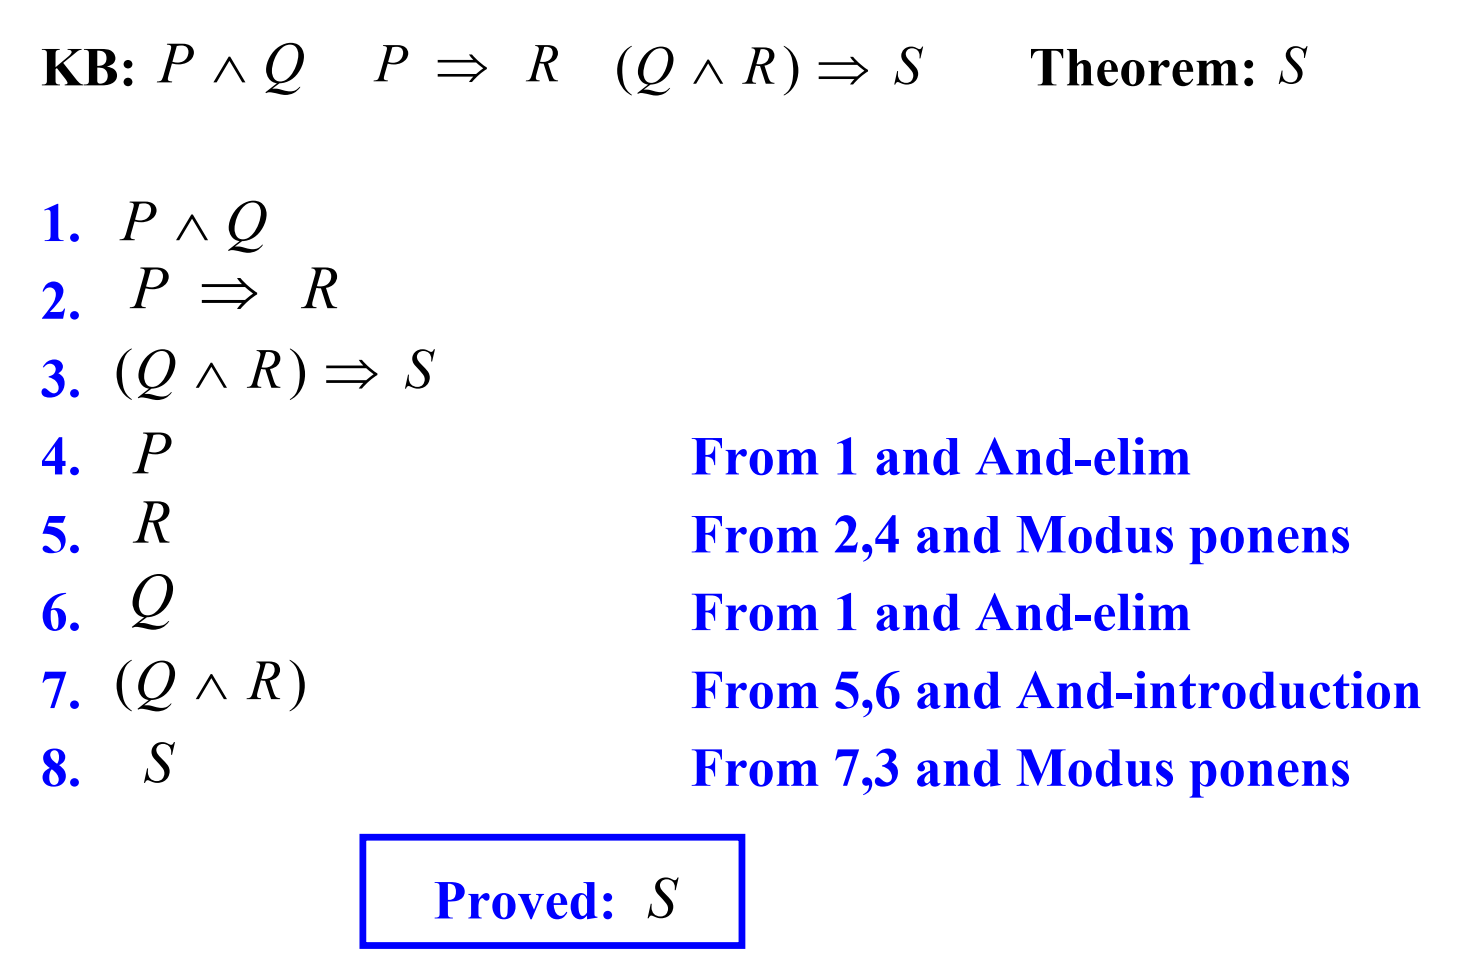
\includegraphics[width=0.4\textwidth]{img/ruleapplication.png}
\end{figure}
This algorithm is sound (inference rules are sound) but it is not complete, unless we define more rules.

There is no way of knowing how many rules do we have to apply or which rule to use at any step.
This can be thought as an instance of a search problem
\subsection{Satisfiability and resolution}
\subsubsection{Validity vs. Satisfiability}
Since we know what we want to prove (i.e we know the Theorem) a clever way would be to find a way to use conclusions in the search for conclusions.

\begin{tcolorbox}[colback=red!5!white,colframe=red!75!black,title=\textbf{Validity Definition}, label=def:validity]
    \label{def:val}
    A formula is valid if it is true in \textbf{all} possible models.
    \begin{equation*}
        \text{For any sentences } \alpha \text{ and } \beta, \alpha \models \beta \text{ if and only if the sentence }\alpha\implies\beta \text{ is valid}
    \end{equation*}
\end{tcolorbox}
\begin{tcolorbox}[label=def:sat,colback=red!5!white,colframe=red!75!black,title=\textbf{Satisfiability Definition}]
    \label{def:sat}
    A formula is satisfiable if it is true in \textbf{at least one} model.
    \begin{itemize}
        \item If f is valid, than the negation of f is unsatisfiable
        \item If f is satisfiable, then the negation of f is invalid
    \end{itemize}
    \begin{equation*}
        \alpha \models \beta \text{ if and only if the sentence }\alpha\land\lnot\beta \text{ is unsatisfiable} \quad \text{\textbf{(Absurdum reduction)}}
    \end{equation*}
    Proving a thesis is equivalent to proving the absurdum of its negation.
\end{tcolorbox}
From Definition of Validity and Satisfiability we can reformulate entailment:
\begin{equation*}
    \alpha\models\beta\;\leftrightarrow\;\alpha\implies\beta\;=\;\lnot\alpha\lor\beta\rightarrow negation \rightarrow \lnot(\lnot\alpha\lor\beta)\rightarrow \alpha\lor\lnot\beta
\end{equation*}
Now we have converted the problem of entailment into proving that a formula is UNSAT.

\subsubsection{Resolution}
Resolution assumes that knowledge base and thesis are expressed in Conjunctive
Normal Form (CNF).
\begin{itemize}
    \item \textbf{Normal form} corresponds to clauses (disjunctions and negations only).
    \item \textbf{CNF} corresponds to conjunction of clauses
\end{itemize}
\section{Answer Set Programming for explainable planning}
\subsection{Planning problem definition in FOL}
\begin{minipage}[t]{0.2\textwidth}
    \begin{figure}[H]
        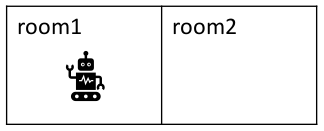
\includegraphics[width=0.9\textwidth]{img/env.png}
        \centering
    \end{figure}
\end{minipage}
\begin{minipage}[t]{0.8\textwidth}
    Given the problem on the left where a robot starting in room A has to change room.\\
    We define the knowledge base in FOL:
    \setstretch{0.5}
    \begin{itemize}
        \item Rooms A, B with possible constant values room1, room2
        \item Location (state) $at(A)$
        \item Action predicate $move(A, B)$
        \begin{itemize}
            \item Precondition: $move(A, B) \leftarrow at(A)$
            \item Effect 1 (post-cond.): $at(B) \leftarrow move(A, B)$
            \item Effect 2: $not\;at(A) \leftarrow move(A, B)$
            \item Constraint: $move(A, B),\;A \ne B$
        \end{itemize}
        \item Initial state: $at(room1)$
        \item Goal state: $at(room2)$
    \end{itemize}
\end{minipage}
\setstretch{1}
\subsubsection*{Model Checking}
To solve the problem with Model Checking we have to first enumetare all possibilites.\\
What's the plan?
\begin{itemize}
    \item Start from the initial state $at(room1)$
    \item Which variables can we substitute (ground) in $move(A, B)$?
    \begin{itemize}
        \item $move(room1, room2)$
        \item $move(room2, room1)$
        \item $move(room1, room1)$
        \item $move(room2, room2)$
    \end{itemize}
\end{itemize}

\vspace*{1pt}
Now knowing that we are $at(room1)$ we can use our \textbf{precondition} to remove actions that violates those.\\

\begin{minipage}[t]{0.5\textwidth}
    \setstretch{0.5}
    \begin{itemize}
        \item Rooms A, B with possible constant values room1, room2
        \item Location (state) $at(A)$
        \item Action predicate $move(A, B)$
        \begin{itemize}
            \item \textcolor{red}{Precondition: $move(A, B) \leftarrow at(A)$}
            \item Effect 1 (post-cond.): $at(B) \leftarrow move(A, B)$
            \item Effect 2: $not\;at(A) \leftarrow move(A, B)$
            \item Constraint: $move(A, B),\;A \ne B$
        \end{itemize}
        \item Initial state: $at(room1)$
        \item Goal state: $at(room2)$
    \end{itemize}
\end{minipage}
\begin{minipage}[t]{0.8\textwidth}
    \begin{itemize}
        \item Start from the initial state $at(room1)$
        \item Which variables can we substitute (ground) in $move(A, B)$?
        \begin{itemize}
            \item $move(room1, room2)$
            \item \textcolor{red}{\st{$move(room2, room1)$}}
            \item $move(room1, room1)$
            \item \textcolor{red}{\st{$move(room2, room2)$}}
        \end{itemize}
    \end{itemize}
\end{minipage}
\newpage
\noindent
Now knowing that we are $at(room1)$ we can use our constraint to remove actions that violates that.\\

\begin{minipage}[t]{0.5\textwidth}
    \setstretch{0.5}
    \begin{itemize}
        \item Rooms A, B with possible constant values room1, room2
        \item Location (state) $at(A)$
        \item Action predicate $move(A, B)$
        \begin{itemize}
            \item \textcolor{red}{Precondition: $move(A, B) \leftarrow at(A)$}
            \item Effect 1 (post-cond.): $at(B) \leftarrow move(A, B)$
            \item Effect 2: $not\;at(A) \leftarrow move(A, B)$
            \item \textcolor{blue}{Constraint: $move(A, B),\;A \ne B$}
        \end{itemize}
        \item Initial state: $at(room1)$
        \item Goal state: $at(room2)$
    \end{itemize}
\end{minipage}
\begin{minipage}[t]{0.8\textwidth}
    \begin{itemize}
        \item Start from the initial state $at(room1)$
        \item Which variables can we substitute (ground) in $move(A, B)$?
        \begin{itemize}
            \item $\bm{move(room1, room2)}$
            \item \textcolor{red}{\st{$move(room2, room1)$}}
            \item \textcolor{blue}{\st{$move(room1, room1)$}}
            \item \textcolor{red}{\st{$move(room2, room2)$}}
        \end{itemize}
    \end{itemize}
\end{minipage}
\setstretch{1}
\vspace{0.5cm}
Now by applying preconditions and constraints we found that the only feasible action is $move(room1, room2)$.
Progating that action we can see that we reach the goal.

\begin{minipage}[t]{0.5\textwidth}
    \setstretch{0.5}
    \begin{itemize}
        \item Rooms A, B with possible constant values room1, room2
        \item Location (state) $at(A)$
        \item Action predicate $move(A, B)$
        \begin{itemize}
            \item \textcolor{red}{Precondition: $move(A, B) \leftarrow at(A)$}
            \item \textcolor{ForestGreen}{Effect 1 (post-cond.): $at(B) \leftarrow move(A, B)$}
            \item Effect 2: $not\;at(A) \leftarrow move(A, B)$
            \item \textcolor{blue}{Constraint: $move(A, B),\;A \ne B$}
        \end{itemize}
        \item Initial state: $at(room1)$
        \item Goal state: $at(room2)$
    \end{itemize}
\end{minipage}
\begin{minipage}[t]{0.8\textwidth}
    \begin{itemize}
        \item Start from the initial state $at(room1)$
        \item Which variables can we substitute (ground) in $move(A, B)$?
        \begin{itemize}
            \item $\bm{move(room1, room2)}$
            \item \textcolor{red}{\st{$move(room2, room1)$}}
            \item \textcolor{blue}{\st{$move(room1, room1)$}}
            \item \textcolor{red}{\st{$move(room2, room2)$}}
        \end{itemize}
    \end{itemize}
\end{minipage}
\setstretch{1}
\vspace{0.1cm}

Which term may I infer? \textcolor{ForestGreen}{$at(room2)$}. This means that we reached the goal and so
$\{move(room1,room2)\}$ is a solution for this planning problem.

\subsubsection*{Absurd Reduction}
\begin{itemize}
    \item KB\footnote{KB also includes axioms, here omitted for simplicity}$=\{at(room1), \underline{at(room2)}, move(room1,room2)\}$
    \item Add goal negation: $KB + \{\underline{not\;at(room2)}\}$
\end{itemize}
Extended KB is contradictory.
Absurdum $\rightarrow \{move(room1,room2)\}$ is ground and solves the planning problem

If we continue progating with the second Effect
% What happens if we add Time?

\begin{minipage}[t]{0.5\textwidth}
    \setstretch{0.5}
    \begin{itemize}
        \item Rooms A, B with possible constant values room1, room2
        \item Location (state) $at(A)$
        \item Action predicate $move(A, B)$
        \begin{itemize}
            \item \textcolor{red}{Precondition: $move(A, B) \leftarrow at(A)$}
            \item \textcolor{ForestGreen}{Effect 1 (post-cond.): $at(B) \leftarrow move(A, B)$}
            \item \textcolor{Dandelion}{Effect 2: $not\;at(A) \leftarrow move(A, B)$}
            \item \textcolor{blue}{Constraint: $move(A, B),\;A \ne B$}
        \end{itemize}
        \item Initial state: $at(room1)$
        \item Goal state: $at(room2)$
    \end{itemize}
\end{minipage}
\begin{minipage}[t]{0.8\textwidth}
    \begin{itemize}
        \item Start from the initial state $at(room1)$
        \item Which variables can we substitute (ground) in $move(A, B)$?
        \begin{itemize}
            \item $\bm{move(room1, room2)}$
            \item \textcolor{red}{\st{$move(room2, room1)$}}
            \item \textcolor{blue}{\st{$move(room1, room1)$}}
            \item \textcolor{red}{\st{$move(room2, room2)$}}
        \end{itemize}
    \end{itemize}
\end{minipage}
\setstretch{1}

KB=$\{\underline{at(room1)}, at(room2), move(room1,room2), \underline{\textcolor{Dandelion}{not\;at(room1)}\}}$

By doing so we reach an Absurdum inside out knowledge base. Which is a problem, to solve this we need to add time.
\vspace{0.5cm}

We define the knowledge base in FOL:
\setstretch{0.5}
\begin{itemize}
    \item Rooms A, B with possible constant values room1, room2
    \item Location (state) $at(A)$
    \item Action predicate $move(A, B)$
    \begin{itemize}
        \item Precondition: $move(A, B, \textcolor{red}{t}) \leftarrow at(A, \textcolor{red}{t})$
        \item Effect 1 (post-cond.): $at(B, \textcolor{red}{t+1}) \leftarrow move(A, B, \textcolor{red}{t})$
        \item Effect 2: $not\;at(A, \textcolor{red}{t+1}) \leftarrow move(A, B, \textcolor{red}{t})$
        \item Constraint: $move(A, B, \textcolor{red}{t}),\;A \ne B$
    \end{itemize}
    \item Initial state: $at(room1, \textcolor{red}{0})$
    \item Goal state: $at(room2, \textcolor{red}{t>0})$
\end{itemize}
\setstretch{1}
With similar reasoning as above:
KB=$\{at(room1, 0), move(room1,room2, 0), not\;at(room1, 1), at(room2, 1)\}$

Resolving with Absurd Reduction: $KB + \{not\;at(room2, 1)\}$ we reach an absurdum

\subsection{Practical implementation of FOL for plan representation and reasoning}
Practical implementations of FOL and logical formalisms, to perform autonomous reasoning and inference, are logic programs.
Several options exist:
\begin{itemize}
    \item Prolog (FOL)
    \item \textbf{Answer Set Programming (FOL)}
    \item Problog (FOL + probability)
    \item Temporal ASP (FOL + LTL)
\end{itemize}
For this course we'll use Answer Set Programming (ASP).
\subsection{Answer Set Programming (ASP)}
A logic programming paradigm specifically intended for planning representation and reasoning.

It contains useful constructs fot planning:
\begin{itemize}
    \item Weak constraints (optimization)
    \item Aggregates (choice among actions)
    \item API interfaces with external programs (e.g., sensors)
    \item Non-monotonic reasoning (plan revision)
    \item Built-in time and goal representation
\end{itemize}

\subsubsection{Syntax}
Variables are marked with capital letter, constants and predicates (or atoms) with lower case.
Constants are either strings or integers.

Example: $move(A, B, T), move(room1, room2, 1)$\\

Logical implications are written with capital and minus signs (:-) with a head body structure (head :- body) 
% where the head implies the body.

Example: $move(A, B, T)$ :- $at(A, T)$\\

Logical Conjunction: is expressed with a comma or a semicolon

Example: $move(A, B, T)$ :- $at(A, T), free(B, T)$ or $move(A, B, T)$ :- $at(A, T); free(B, T)$\\

Logical negation: is expressed with a minus sing

Example: $-at(A, T+1)$ :- $move(A, B, T)$\\

Default negation: also called Negation As Failure(NAF)

Example: $not\;at(A, T+1)$ :- $move(A, B, T)$\\

\subsection{Two negations}

\begin{table}[H]
    \centering
    \begin{tabular}{cclcc}
    \multicolumn{2}{c}{{\color[HTML]{000000} \textbf{Logic Negation}}} &  & \multicolumn{2}{c}{\textbf{Negation As Failure}}             \\
    {\color[HTML]{FD6864} $p$}      & {\color[HTML]{FD6864} $-p$}      &  & {\color[HTML]{FD6864} $p$} & {\color[HTML]{FD6864} $not\;p$} \\
    0 & 1 &  & 0 & 1 \\
    1 & 0 &  & 0 & 1 \\
    ? & ? &  & ? & 0
    \end{tabular}
\end{table}

\begin{itemize}
    \item \textbf{Logic (classical or Boolean) negation}:\\
    p may be an observation, hence it may be unknown (e.g., in robotic navigation)

    \item  \textbf{Negation As Failure (NAF)}:\\
    if $p$ is unknown we set it to false by default
\end{itemize}

\textbf{Why NAF?}
Real World is characterized by Incomplete observations. If the agent does not know (observe) something, he could get stuck!
NAF allows to reason on default if a fact is unknown, assume it is false by default.

This behaviour is called \emph{Closed-World Assumption (CWA)}, this simple assumption states that if I don't know something, it is not important.\\

The planning scenario is typically dynamic (the environment may change, new observations may be acquired...).
So if we use the $CWA$ once we'll discover new information we'll update our knowledge.\\

This is possible only if the knowledge base (and related logic formalism) is \textbf{non-monotonic}.

\begin{itemize}
    \item \textbf{Monotonic KB (and formalism)}
    \begin{itemize}
        \item Given K and A, if $K \models A$ then $K \cup S \models A$ \textbf{for all S} (additional knowledge or
        rules)
    \end{itemize}
    \item \textbf{Non-monotonic KB (and formalism)}
    \begin{itemize}
        \item Given K and A, if $K \models A$ then $K \cup S \models A$ \textbf{may not hold for some S} (additional knowledge or rules)
        \item This is called Knowledge revision (dynamic knowledge)
    \end{itemize}
\end{itemize}

\subsubsection{Structure of ASP program}
In an ASP program, variables are defined like this:
\begin{itemize}
    \item Range of variables: $room(room1; room2)\quad time(1..10)$
    \item A generic room variable as an atom: $room(A)$
    \item Typically, we start an ASP program defining ranges of variables
\end{itemize}
We can also define facts, i.e., atoms with no variables
\begin{itemize}
    \item $closed\_door$
\end{itemize}

A rule, or axiom, must be safe, i.e., \textbf{all variables in the head must appear also in the body without negation nor NAF}
Examples:
\begin{itemize}
    \item $move(A, B)$ :- $not\;closed\_door, at(A)$ \cross
    \item $move(A, B)$ :- $not\;closed\_door, at(A), room(B)$ \tick
    \item $move(A, B, T)$ :- $not\;closed\_door, at(A), room(B)$ \cross
    \item $move(A, B, T)$ :- $not\;closed\_door(T), at(A, T), room(B)$ \tick
    \item $move(A, B, T)$ :- $not\;closed\_door(T)$ \cross
\end{itemize}

In ASP we can define Hard constraints\\
$move(A, B)$ :- $not\;closed\_door, room(A), room(B)$ \\
can be rewritten as...\\
:- $move(A, B), closed\_door$\\

A rule with empty head is a hard constraint (or just constraint)

:- $body$ is equivalent to $\perp$(Falsum) :- body (i.e., the body atoms cannot hold concurrently, they must lead to UNSAT or inconsistency)\\

In ASP we can also define aggregates\\
$l\;\{h1(:b1); h2(:b2), \ldots\}\;u$

A set of axioms (or facts, i.e., axioms without body). $h1 : b1$ is semantically equivalent to $h1$ :- $b1$ (which is not allowed in aggr.)

The aggregate specifies that at least $l$ and at most $u$ head atoms can be returned (grounded) from the aggregate.\\

% \begin{minipage}[t]{0.2\textwidth}
%     \begin{figure}[H]
%         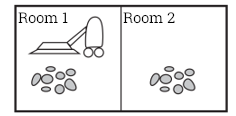
\includegraphics[width=\textwidth]{img/vacum.png}
%     \end{figure}
% \end{minipage}
% \begin{minipage}[t]{0.8\textwidth}
%     An Example for planning $l\;\{h1(:b1); h2(:b2), \ldots\}\;u$

%     \begin{itemize}
%         \item $move(A,B,T)$ :- $at(A,T), room(B)$
%         \item $suck(T)$ :- $at(A,T), dirty(A,T)$
%         \item Init:$at(room1,0), dirty(room1,0), dirty(room2,0)$
%         \item KB=$\{at(room1,0), dirty(room1,0), dirty(room2,0),move(room1,room2,0), suck(0)\}$
%     \end{itemize}
% \end{minipage}

ASP implements a fragment of FOL. We may need some temporal expressiveness in a planning domain.

$X\varphi$ is expressed as $at(B,T+1)$ :- $move(A,B,T)$

The robot's location does not change \textbf{until} it moves, $at(A)\; U\;move(A,B), A!=B$



\tikzset{every picture/.style={line width=0.75pt}} %set default line width to 0.75pt        

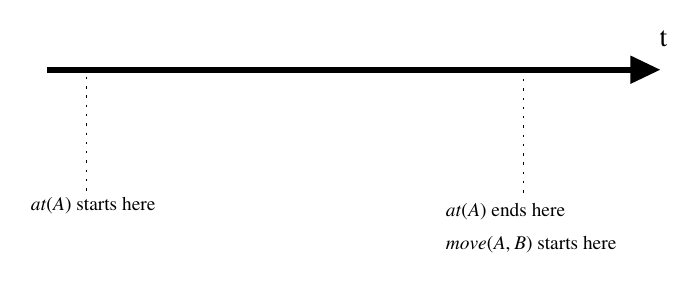
\begin{tikzpicture}[x=0.75pt,y=0.75pt,yscale=-1,xscale=1]
%uncomment if require: \path (0,469); %set diagram left start at 0, and has height of 469

%Straight Lines [id:da6944126603890698] 
\draw [line width=2.25]    (131,92) -- (421.42,92) ;
\draw [shift={(426.42,92)}, rotate = 180] [fill={rgb, 255:red, 0; green, 0; blue, 0 }  ][line width=0.08]  [draw opacity=0] (14.29,-6.86) -- (0,0) -- (14.29,6.86) -- cycle    ;
%Straight Lines [id:da04455549601993869] 
\draw  [dash pattern={on 0.84pt off 2.51pt}]  (150,91) -- (150,153.08) ;
%Straight Lines [id:da3086215716473073] 
\draw  [dash pattern={on 0.84pt off 2.51pt}]  (360.71,92) -- (360.71,154.08) ;

% Text Node
\draw (122,152) node [anchor=north west][inner sep=0.75pt]   [align=left] {{\scriptsize $\displaystyle at( A)$ starts here}};
% Text Node
\draw (322,155) node [anchor=north west][inner sep=0.75pt]   [align=left] {{\scriptsize $\displaystyle at( A)$ ends here}\\{\scriptsize $\displaystyle move( A,B)$ starts here}};
% Text Node
\draw (425,72) node [anchor=north west][inner sep=0.75pt]   [align=left] {t};

\end{tikzpicture}

\begin{itemize}
    \item $at(A,T)$ :- $init(at(A),T)$
    \item $at(A,T)$ :- $at(A,T-1), not\; term(at(A),T)$
    \item $move(A,B,T)$ :- $init(move(A,B),T)$
\end{itemize}

Instead of saying until we say at time $t$ something starts holding, until something else occurs it holds.
In between it continues holding.

This assumption is called $INERTIA$

\subsubsection{ASP reasoning}
So far, we have seen main syntax and semantics of ASP.

How do we perform reasoning in ASP? Hence, how can an ASP program actually produce a plan?

To this there exist two main phases:
\begin{itemize}
    \item Grounding
    \item Solving (reasoning in propositional logic)
\end{itemize}

\textbf{Grounding}

Apply a substitution to variables, depending on initial conditions and propagating through axioms (let's do it for $T<2$ for simplicity).\\

$room(room1;room2)$\\
$at(room1,0)$\\
$closed\_door(0)$\\
$move(A,B,T)$ :- $at(A,T), room(B)$\\
$init(at(A),T)$ :- $move(B,A,T-1)$\\
$term(at(A),T)$ :- $move(A,B,T-1), A\ne B$\\
$at(A,T)$ :- $init(at(A),T)$\\
$at(A,T)$ :- $at(A,T-1), not term(at(A),T)$\\
:- $move(A,B,T), closed\_door(T)$\\
:- $not\;at(room2,1)$ (GOAL AS CONSTRAINT)\\

Substitute
$A=room1,\;B=room2,\;T=0,1$\\

$room(room1)\;room(room2)$\\
$at(room1,0)$\\
$closed\_door(0)$\\
$move(room1,room2,0) \leftarrow at(room1,0), room(room2)$\\
$init(at(room2),1) \leftarrow move(room2,room1,0)$\\
$term(at(room1),1)  \leftarrow move(room1,room2,0), room1\ne room2$\\
$at(room2,0)$ :- $init(at(room2),1)$\\
$Falsum \leftarrow move(room1, room2,0), closed\_door(0)$\\
$Falsum \leftarrow not\;at(room2, 1)$\\

Ground atoms become True Booleans (facts)! The set of all possible groundings is also known as Herbrand universe of program.

\newpage
The goal of an answer set solver, given a ground program, is to compute the answer sets (or stable models) of it.

Given a ground knowledge base KB, a \textbf{stable model} of KB is a \textbf{minimal set} of True Booleans (facts) \textbf{satisfying} KB.

\subsubsection{ASP reasoning in practice}
In practice Solving is an instance of Conflict-Driven Constraint Learning for SAT checkin.

Grounding is Exp Time Hard and its one of the main bottleneks, there are some assumptions that help
mitigating the complexity like Safe Axioms which helps reducing the number of possible groundings.
\section{Inductive learning of logical (task) rules}
In real life it may be hard to express the planning problem explicitly.

In partincular defining the precondition and the constraints of actions is challenging.

Looking at the classical Reinforcement Learning loop:
\begin{figure}[H]
    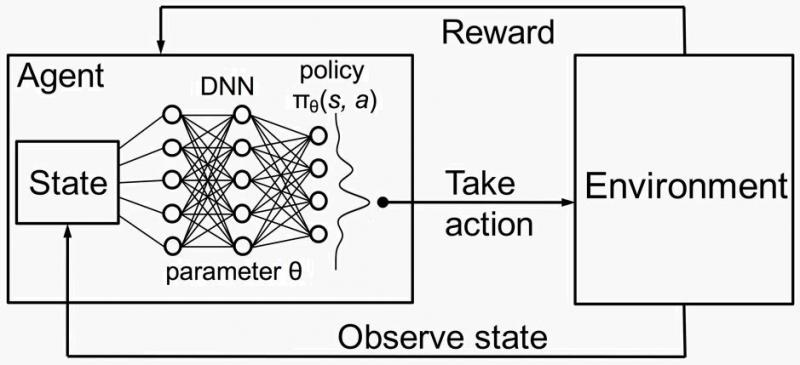
\includegraphics[width=0.5\textwidth]{img/RL.png}
    \centering
\end{figure}

RL is typically used to learn a state-action map (policy), given:
\begin{itemize}
    \item Transition model
    \item Reward model (hence goal)
    \item State and action spaces definition
    \item (possibly observation model under partial observability)
\end{itemize}

So in this context preconditions are logical representations of the policy mapping 
but Neural Networks are black box models.

However, we need explainable (or at least interpretable) models of agency in critical scenarios for trust and legal requirements.\\

When we execute the policy we know the state in which the agent is and the action taken by the agent.
One option could be to use Causal Discovery where State and action can be represented as time series so we want to find the causal relation between the state and the action.
The problem is that Causal Discovery outputs pairwise relations but those may not be expressive enough.

A more powerful approach would be to start from a logical formalization 
of the state and variables and then learn logical rules which can be used as a logical representation of the policy.
This task is usually known as \emph{Inductive logic programming}.

\subsection{Inductive logic programming}
Usually in Deductive Reasoning(what we've seen so far) we start from a Knowledge Base and we derive consequences of it.
In Inductive Reasoning we start from facts and we try to infer the logical rules which actually lead to that.

In Inductive logic programming we need to define:
\begin{itemize}
    \item \textbf{State-action pairs} (i.e examples) which may be Positive and Negatives
    \item \textbf{Background knowledge} which are known facts and axioms
    \item Set of possible rules(actions), or \textbf{search space}
\end{itemize}

The main definition of Inductive logic programming is Learning from entailment.
\begin{tcolorbox}[colback=red!5!white,colframe=red!75!black,title=\textbf{Definition 4: Learning from entailment}]
Consider a set of examples $E=\langle E^+,E^- \rangle$, where $E^+$ is a subset of positive examples and $E^-$ is a subset of negative examples.
The task of learning from entailment is defined as the tuple $T=\langle B, S_M, E \rangle$. THe goal of $T$ is to find $H\subseteq S_M$ such that:
\begin{itemize}
    \item $B\;\cup\;H\models E^+$
    \item $B\;\cup\;H\;\cup\;E^-\models \bot$
\end{itemize}
\end{tcolorbox}
This means that we want to learn $H$(called hypotesis) that supports our positive
examples (i.e if we add the hypotesis to the Background knowledge $B$ we can entail
the positive examples) and that does not support (is in contraddiction with) the negative
examples (i.e if we add together the negative hypotesis, the background knowledge and the
negative examples we reach a contraddiction).\\

To understand better let's go back to the classical robot changing room example:\\

\begin{minipage}[t]{0.2\textwidth}
    \begin{figure}[H]
        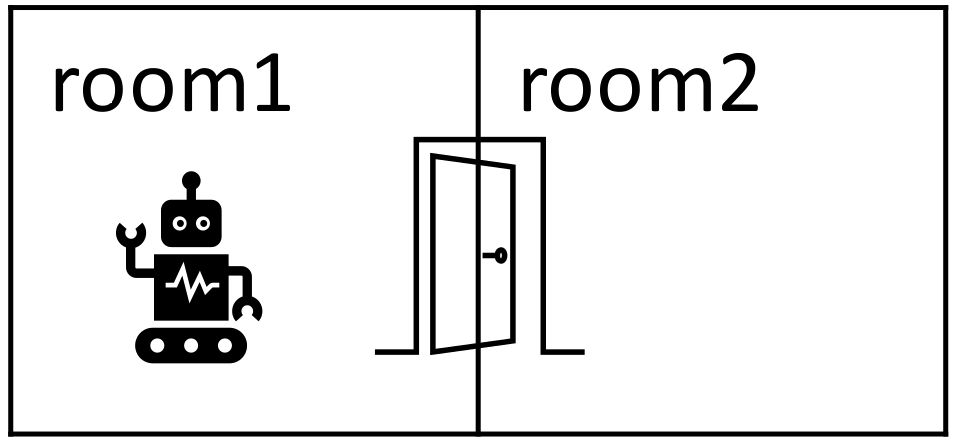
\includegraphics[width=\textwidth]{img/robot_room.png}
        \centering
    \end{figure}
\end{minipage}
\begin{minipage}[t]{0.8\textwidth}
    \begin{itemize}
        \item $E^+ = \{move(room1,room2,0), at(room1,0),
        not\;closed\_door(0), not\;closed\_door(1),
        at(room2,1)\}$
        \item $\{move(room2,room1,0)\}$
        \item $B = \{room(room1), room(room2), at(A,T) \leftarrow move(A,B,T-1), time(0..N)\}$
        \item $S_{M}=\{\\
                move(A,B,T) \leftarrow closed\_door(T); \\
                move(A,B,T) \leftarrow at(A,T);\\
                move(A,B,T) \leftarrow at(A,T), not\;closed\_door(T);\\
                \ldots\} \; \text{and all possible combinations}$
    \end{itemize}
\end{minipage}

\vspace{0pt}
If we apply learning from entailment here, we can learn the following hypotesis:\\
$H = \{move(A,B,T) \leftarrow at(A,T)\}\;\text{OR}\;\{move(A,B,T)\leftarrow at(A,T), not\;closed\_door(T)\}$.\\

Those are only some examples since multiple hypotheses can be found.
We are observing a limited number of task realizations we will never be sure to capture correct and complete knowledge!

\begin{tcolorbox}[colback=red!5!white,colframe=red!75!black,title=\textbf{Definition 5: Partial interpretation}]
Let $P$ be an ASP program. Any set of ground atoms that can be generated from axioms in $P$ is an interpretation of $P$.
Given an interpretation $I$ of $P$, a pair of subset of ground atoms $e=\langle e^{inc}, e^{exc}\rangle$ is said to be a partial
interpretation extended by interpretation $I$ if $e^{inc} \subseteq I$ and  $e^{exc} \cap I = \emptyset.$
\end{tcolorbox}

Given the previous definition an Answer Set can be sayed to be an interpretation since an Answer Set is definied as 
the minimal set of ground atoms which can be generated from the problem.
Also given the interpretation we can define also a partial interpretation which means a coupled subsets of ground atoms which we 
denote as the included set (\textcolor{Green}{$e^{inc}$}) and the excluded set (\textcolor{Red}{$e^{exc}$}) where the first is part
(i.e a subset) of the interpretation and the later has nothing in common with the Interpretation\\

If we start from an interpretation $I$:
\begin{equation*}
    I = AS = \{room(room1), room(room2), move(room1,room2,0), at(room1,0), at(room2,1), init(at(room2),1), \ldots\}
\end{equation*}
Some partial interpretation are:
\begin{align*}
    e1 &= \langle\textcolor{Green}{\{move(room1,room2,0), at(room1,0),at(room2,1)\}},\; \textcolor{Red}{\{move(room2,room1,0)\}}\rangle;\\
e2 &= \langle\textcolor{Green}{\{move(room1,room2,0), at(room1,0)\}},\;\textcolor{Red}{\{\}}\rangle
\end{align*}

Before we can move to learning Answer Set Programming we need to define other two definitions which are two substasks of learning from induction.
\begin{tcolorbox}[colback=red!5!white,colframe=red!75!black,title=\textbf{Definition 6: Brave Induction task}]
Let $\mathcal{T}=\langle B,S_M, E\rangle$, $H$, and $E=\langle E^+,E^- \rangle$ be as defined for learning from entailment 
under the AS semantics. Let $A$ be an answer set of the ASP program defined by $H \cup B$.
$\mathcal{T}$ is said to define a brave induction task if the goal set $H$ of hypotesis must satisfy:
\begin{equation*}
    \exists A\;s.t\;B \cup H \entails A: A\cap E^- =\emptyset\;\land\;E^+\subseteq A
\end{equation*}
\end{tcolorbox}

In this task we want to find an hypotesis which generates at least one answer set which excludes negative 
examples and entails positive examples.Positive examples should be entailed by \textbf{at least an answer set}
and Negative examples should be not entailed by \textbf{at least an answer set}.\\

The opposite of Brave Induction is the Cautious Induction:
\begin{tcolorbox}[colback=red!5!white,colframe=red!75!black,title=\textbf{Definition 7: Cautious induction task}]
    Let $\mathcal{T}=\langle B,S_M, E\rangle$, $H$, and $E=\langle E^+,E^- \rangle$ be as defined for learning from entailment 
    under the AS semantics. Let $A$ be an answer set of the ASP program defined by $H \cup B$.
    $\mathcal{T}$ is said to define a cautious induction task if the goal set $H$ of hypotesis must satisfy:
    \begin{equation*}
        \forall A\;s.t\;B \cup H \entails A: A\cap E^- =\emptyset\;\land\;E^+\subseteq A
    \end{equation*}
\end{tcolorbox}

Contrary to the brave induction Positive examples should be entailed by \textbf{all answer sets} and Negative examples should be not entailed by
\textbf{any answer set}

\subsection{Inductive learning of answer set programs (ILASP)}
Given the previous definitions we can give the definion of Inductive learning of answer set programs which is a particular specialization
of Learning from Entailment task.

\begin{tcolorbox}[colback=red!5!white,colframe=red!75!black,title=\textbf{Definition}]
The ILASP learning task $\mathcal{T}=\langle B,S_M, E\rangle$ is a tuple of background knowledge $B$, search space $S_M$ and examples $E=\langle E^+,E^- \rangle$ 
such that $E^+ (E^-)$ is the subset of positive (negative) examples. The goal of $\mathcal{T}$ is to find $H \subseteq S_M$ such that $\forall e\in E$, $e$ is a 
particular interpretation of the ASP program $B\cup H$. If AS is an answer set of the ASP program $H\cup B$ the following must hold:
\begin{align*}
    \forall e \in E^+\exists AS\;s.t\; B\cup H\entails AS: e \;\text{is extended by AS}\\
    \forall e \in E^-\cancel{\exists} AS\;s.t\; B\cup H\entails AS: e \;\text{is extended by AS}
\end{align*}
\end{tcolorbox}

The ILASP task is a combination of brave and cautious tasks. 
The goal of ILASP task is to find an hypotesis which satisfies this two conditions:
\begin{itemize}
    \item Positive examples should be entailed by \textbf{at least an answer set} (brave)
    \item Negative examples should be not entailed \textbf{by any answer set} (cautious)
\end{itemize}
In this task examples are structured as partial interpretations.\\

For the sake of this course we are particularly interested in ILASP under CDPIs (context-dependent partial interpretations).
\begin{tcolorbox}[colback=red!5!white,colframe=red!75!black,title=\textbf{Definition 3: Context-dependent partial interpretation (CDPI)}]
A CDPI of an ASP program $P$ with an interpretation $I$ is a tuple $e_c=\langle e, C\rangle = \langle e^{inc},e^{exc}, C\rangle$, where $e$ is a partial interpretation, and $C$ is an 
ASP program called $context$. $I$ is said to extend $e_c$ if $e^{inc}\cup C\subseteq I$ and $(e^{exc}\cup C) \cap I = \emptyset$
\end{tcolorbox}

\begin{tcolorbox}[colback=red!5!white,colframe=red!75!black,title=\textbf{Definition 4: ILASP task with CDPIs}]
An ILASP learning task with CDPIs is a tuple $\mathcal{T}=\langle B,S_M, E\rangle$, where $E=\langle E^+,E^- \rangle$ is a set of CDPIs
with context $C$. We say that $H\subseteq S_M$ is a solution to $\mathcal{T}$ if the following hold:
\begin{align*}
    \forall e \in E^+\exists AS\;s.t\; B\cup H\cup C\entails AS: e \;\text{is extended by AS}\\
    \forall e \in E^-\cancel{\exists} AS\;s.t\; B\cup H\cup C\entails AS: e \;\text{is extended by AS}
\end{align*}
\end{tcolorbox}

To understand better let's go back to our usual example:\\

\begin{minipage}[t]{0.2\textwidth}
    \begin{figure}[H]
        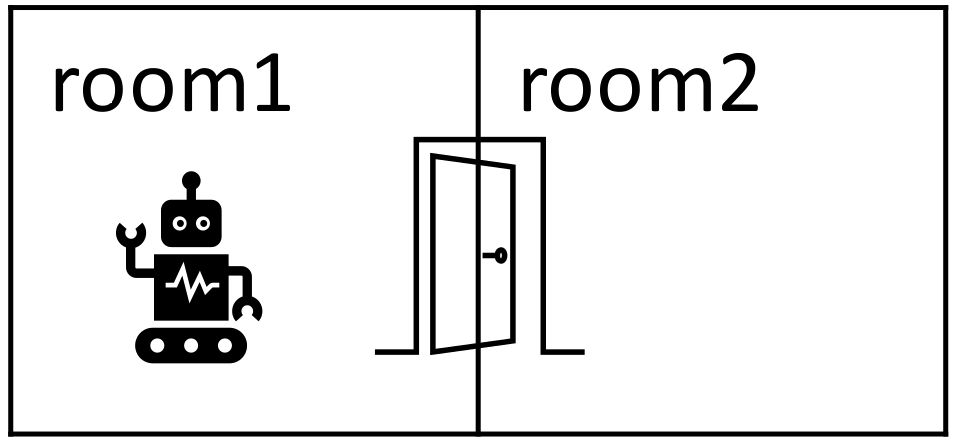
\includegraphics[width=\textwidth]{img/robot_room.png}
        \centering
    \end{figure}
\end{minipage}
\begin{minipage}[t]{0.8\textwidth}
    \begin{itemize}
        \item $\textcolor{Blue}{e^{inc}},\textcolor{Green}{e^{exc}},\textcolor{Red}{C}$
        \item $E^+ = \langle\{\textcolor{Blue}{move(room1,room2,0)}\},\textcolor{Green}{\{\}}, \{\textcolor{Red}{at(room1,0),at(room2,1)}\}\rangle$
        \item $E^- = \langle\{\textcolor{Blue}{move(room2,room1,0)}\},\textcolor{Green}{\{\}}, \{\textcolor{Red}{at(room1,0),at(room2,1)}\}\rangle$
        \item $B = \{room(room1), room(room2), at(A,T) :-\; move(A,B,T-1), time(0..N)\}$
        \item $S_{M}=\{\\
                    move(A,B,T) :-\; closed\_door(T), room(A), room(B). \\
                    move(A,B,T) :-\; at(A,T), room(B).\\
                    \text{:-}\; move(A,B,T), closed\_door(T).\\
                    \ldots\} \;$
    \end{itemize}
\end{minipage}

We still have positive and negative examples but we split our observations into Excluded and Included sets.
Particularly actions are placed into the included set and the rest of the atoms into the context.
Similarly for the negative examples we have that the included set contains not executed actions  and the rest of the atoms into the context.

This is done because in ILASP we want to discover action preconditions.
Doing so we have that actions(possible heads of hypothesis) and the context (possible body) are separated.\\

A possible hypotesis which satisfies the ILASP task condition is:
\begin{equation*}
    H = \{move(A,B,T) :- at(A,T), room(B).\}
\end{equation*}

Until now we've had an empty excluded set, so why do we need it?

Assume we don't have negative examples but I add something to the excluded set in the positive example:
\begin{itemize}
    \item $E^+ = \{\{move(room1,room2,0)\},\{\textbf{move(room2,room1,0)}\}, \{at(room1,0),at(room2,1)\}\}$
    \item $E^- = \langle\{\},\{\},\{\}\rangle$
    \item $B = \{room(room1), room(room2), at(A,T) :-\; move(A,B,T-1), time(0..N)\}$
    \item $S_{M}=\{\\
                move(A,B,T) :-\; closed\_door(T), room(A), room(B). \\
                move(A,B,T) :-\; at(A,T), room(b).\\
                move(A,B,T) :-\; at(A,T), closed\_door(T);\\
                \ldots\} \;$
\end{itemize}
In this case the Hypotesis will be the same as before.\\

Now lets consider the three romms environment:

\begin{minipage}[t]{0.2\textwidth}
\begin{figure}[H]
    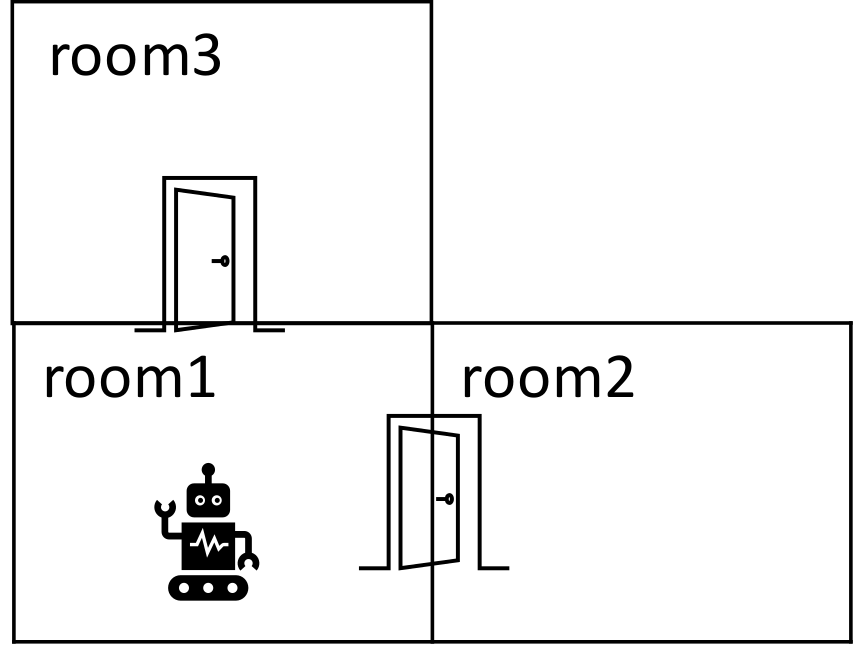
\includegraphics[width=0.9\textwidth]{img/three_room.png}
    \centering
\end{figure}

\end{minipage}
\begin{minipage}[t]{0.8\textwidth}
    $room(room1;room2).\\
    at(room1,0).\\
    closed\_door(0).\\
    0\;\{move(A,B,T) : at(A,T), room(B)\}\;1.\\
    init(at(A),T) \text{:-}\; move(B,A,T-1).\\
    term(at(A),T) \text{:-}\; move(A,B,T-1), A!=B.\\
    at(A,T) \text{:-}\; init(at(A),T).\\
    at(A,T) \text{:-}\; at(A,T-1), not\;term(at(A),T).\\
    \text{:-}\; move(A,B,T), closed\_door(T).\\
    \text{:-}\; not\;at(room2,1), not\;at(room3,1).\\
    AS1 = \{room(room1), room(room2), \ldots, move(room1,room2,0)\}\\
    AS2 = \{room(room1), room(room2), \ldots, move(room1,room3,0)\}$
\end{minipage}\\

If we formalize this into a ILASP task:
\begin{itemize}
    \item $E^+ = \{\{move(room1,room2,0)\},\{\textbf{move(room1,room3,0)}\}, \{at(room1,0),at(room2,1)\}\}$
    \item $E^- = \langle\{\},\{\},\{\}\rangle$
    \item $B = \{room(room1), room(room2), at(A,T) :-\; move(A,B,T-1), time(0..N)\}$
    \item $S_{M}=\{\\
                move(A,B,T) :-\; closed\_door(T), room(A), room(B). \\
                move(A,B,T) :-\; at(A,T), room(B).\\
                \text{:-}\; move(A,B,T), closed\_door(T).\\
                0\;\{move(A,B,T) : at(A,T), room(B)\}\;1\\
                \ldots\} \;$
\end{itemize}
we can learn two hypotesis:
\begin{itemize}
    \item $H = \{move(A,B,T) :- at(A,T), room(B).\}$
    \item $H = \{0\; \{move(A,B,T) : at(A,T), room(B).\}\; 1\}$
\end{itemize}

If we remove the excluded set and add again the negative example:
\begin{itemize}
    \item $E^+ = \{\{move(room1,room2,0)\},\{\}, \{at(room1,0),at(room2,1)\}\}$
    \item $E^- = \langle\{\textbf{move(room1,room3,0)}\},\{\},\{at(room1,0),at(room2,1)\}\rangle$
    \item $B = \{room(room1), room(room2), at(A,T) :-\; move(A,B,T-1), time(0..N)\}$
    \item $S_{M}=\{\\
                move(A,B,T) :-\; closed\_door(T), room(A), room(B). \\
                move(A,B,T) :-\; at(A,T), room(B).\\
                \text{:-}\; move(A,B,T), closed\_door(T).\\
                0\;\{move(A,B,T) : at(A,T), room(B)\}\;1\\
                \ldots\} \;$
\end{itemize}
We have that the second hypotesis is no longer valid:
\begin{itemize}
    \item $H = \{move(A,B,T) \text{:-} at(A,T), room(B).\}$
    \item\st{$H = \{0\; \{move(A,B,T) : at(A,T), room(B).\}\; 1\}$}
\end{itemize}
Because there must be no answer set which extends the negative example.
So the differnce between Negative examples and excluded set stands in the 
different learning task which ilasp performs for positive and negative examples:
\begin{itemize}
    \item Positive examples $\rightarrow$ Brave Induction
    \item Negative examples $\rightarrow$ Cautious Induction
\end{itemize}

Usually what we do when creating an ILASP task is placing the observations in 
the positive examples and use the negative examples only when we want to enforce some safety constraints.\\

Going back to the Reinforcement Learning setting we stated at the beggining,
in this setting we know only about the observations we get and so Negative examples cannot be easily built.

\subsection{ILASP in practice}

\part{Interpretable Machine Learning - Gloria Menegaz}
\section{Interpretability}

It is difficult to (mathematically) define interpretability. A (non-mathematical) definition of interpretability by \cite{miller2019explanation} is:
"\textbf{Interpretability is the degree to which a human can understand the cause of a decision}".

Another one from \cite{kim2016examples} is: "\textbf{Interpretability is the degree to which a human can consistently predict the model's result}".
The higher the interpretability of a machine learning model, the easier it is for someone to comprehend
why certain decisions or predictions have been made. A model is better interpretable than another model 
if its decisions are easier for a human to comprehend than decisions from the other model. 
I will use both the terms interpretable and explainable interchangeably.
\subsection{Importance of Interpretability}
If a machine learning model performs well, why do we not just trust the model and ignore why it made a 
certain decision? “The problem is that a single metric, such as classification accuracy, is an incomplete 
description of most real-world tasks.”\\

Let us dive deeper into the reasons why interpretability is so important.
When it comes to predictive modeling, you have to make a trade-off: 
Do you just want to know what is predicted? For example, the probability that 
a customer will churn or how effective some drug will be for a patient. 
Or do you want to know why the prediction was made and possibly pay for the interpretability 
with a drop in predictive performance? In some cases, you do not care why a decision was made, 
it is enough to know that the predictive performance on a test dataset was good. But in other cases, 
knowing the `why` can help you learn more about the problem, the data and the reason why a model might fail. 
Some models may not require explanations because they are used in a low-risk environment, meaning a mistake 
will not have serious consequences, (e.g. a movie recommender system) or the method has already 
been extensively studied and evaluated (e.g. optical character recognition). 
The need for interpretability arises from an incompleteness in problem formalization, which means that 
for certain problems or tasks it is not enough to get the prediction (the what). 
The model must also explain how it came to the prediction (the why), because a correct prediction 
only partially solves your original problem.\\

Machine learning models take on real-world tasks that require safety measures and testing. 
Imagine a self-driving car automatically detects cyclists based on a deep learning system. 
You want to be 100\% sure that the abstraction the system has learned is error-free, because 
running over cyclists is quite bad. An explanation might reveal that the most important 
learned feature is to recognize the two wheels of a bicycle, and this explanation helps 
you think about edge cases like bicycles with side bags that partially cover the wheels.\\

By default, machine learning models pick up biases from the training data. 
This can turn your machine learning models into racists that discriminate against 
underrepresented groups. Interpretability is a useful debugging tool for detecting 
bias in machine learning models. It might happen that the machine learning model you have 
trained for automatic approval or rejection of credit applications discriminates against a 
minority that has been historically disenfranchised. 
Your main goal is to grant loans only to people who will eventually repay them. 
The incompleteness of the problem formulation in this case lies in the fact that 
you not only want to minimize loan defaults, but are also obliged not to discriminate 
on the basis of certain demographics. This is an additional constraint that is part of 
your problem formulation (granting loans in a low-risk and compliant way) that is not 
covered by the loss function the machine learning model was optimized for.\\

Machine learning models can only be debugged and audited when they can be interpreted. 
Even in low risk environments, such as movie recommendations, the ability to interpret 
is valuable in the research and development phase as well as after deployment.
Later, when a model is used in a product, things can go wrong. \textbf{An interpretation 
for an erroneous prediction helps to understand the cause of the error}.
It delivers a direction for how to fix the system. Consider an example of a 
husky versus wolf classifier that misclassifies some huskies as wolves.

\begin{figure}[H]
    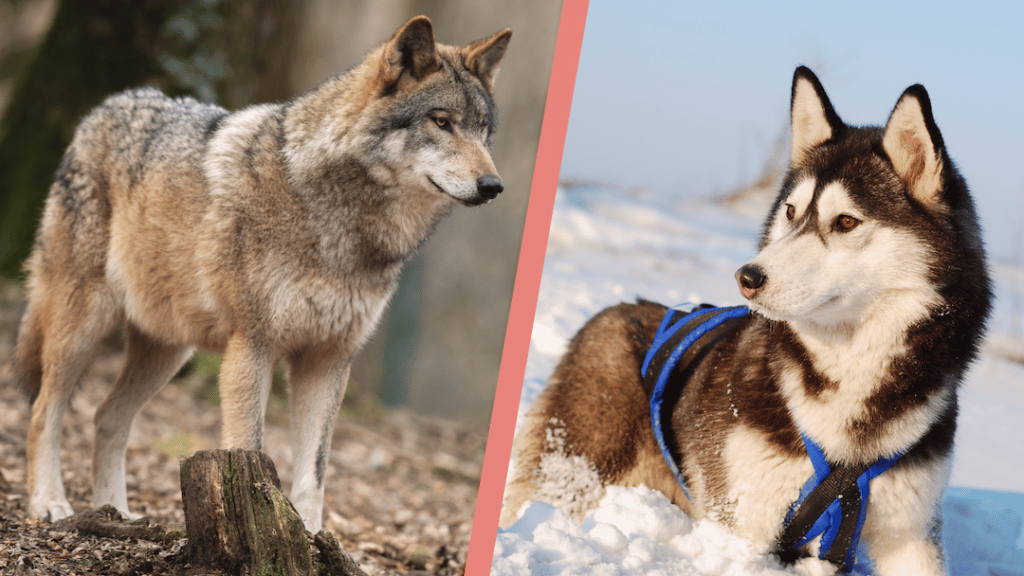
\includegraphics[width=0.5\textwidth]{img/wolf_vs_husky.png}
    \centering
\end{figure}

Using interpretable machine learning methods, you would find that the 
misclassification was due to the snow on the image. 
The classifier learned to use snow as a feature for classifying images as “wolf”, 
which might make sense in terms of separating wolves from huskies in the training 
dataset, but not in real-world use.


\section{Taxonomy of Interpretability Methods}
Methods for machine learning interpretability can be classified according to various criteria.
One of them is the distinction between \textbf{Intrinsic and Post hoc} methods.
\begin{itemize}
    \item \textbf{Intrinsic} $\rightarrow$ Intrinsically explainable models are
    self-explaining. Do not require post-hoc methods though these could be
    applied. Those methods refers to machine learning models that are considered interpretable 
    due to their simple structure, such as short decision trees or sparse linear models.

    \item \textbf{Post hoc} $\rightarrow$ are methods that analyze the model after training and usually model agnostic.
    Assign values to features (attributions, relevance, importance) expressing the impact of the features on the models outcomes.
    Those tecniques can be subdived into two main categories:
    \begin{itemize}
        \item \textbf{Feature importance methods} like for example SHAP, LIME and feature permutation
        \item \textbf{Feature visualization methods} like gradient-based methods
    \end{itemize}
\end{itemize}

Result of the various interpretation methods can be roughly differentiated according to their results:
\begin{itemize}
    \item \textbf{Feature summary statistic} $\rightarrow$ any interpretation methods provide summary 
    statistics for each feature. Some methods return a single number per feature, such as feature importance, 
    or a more complex result, such as the pairwise feature interaction strengths, which consist of a number 
    for each feature pair. 

    \item \textbf{Feature summary visualization} $\rightarrow$ Most of the feature summary statistics can also be visualized. 
    Some feature summaries are actually only meaningful if they are visualized and a table would be a wrong choice. 
    The partial dependence of a feature is such a case. 
    Partial dependence plots are curves that show a feature and the average predicted outcome. 
    The best way to present partial dependences is to actually draw the curve instead of printing the coordinates.

    \item \textbf{Model internals} $\rightarrow$ The interpretation of intrinsically interpretable models falls into this category. 
    Examples are the weights in linear models or the learned tree structure (the features and thresholds used for the splits) 
    of decision trees. The lines are blurred between model internals and feature summary statistic in, for example, linear models, 
    because the weights are both model internals and summary statistics for the features at the same time. Another method that 
    outputs model internals is the visualization of feature detectors learned in convolutional neural networks. Interpretability 
    methods that output model internals are by definition model-specific.

    \item \textbf{Data point} $\rightarrow$  This category includes all methods that return data points (already existent or newly created) 
    to make a model interpretable. One method is called counterfactual explanations. To explain the prediction of a data instance, the method 
    finds a similar data point by changing some of the features for which the predicted outcome changes in a relevant way (e.g. a flip in the 
    predicted class). Another example is the identification of prototypes of predicted classes. To be useful, interpretation methods that output 
    new data points require that the data points themselves can be interpreted. This works well for images and texts, but is less useful for tabular 
    data with hundreds of features.

    \item \textbf{Surrogate models} $\rightarrow$ One solution to interpreting black box models is to approximate them (either globally or locally) with an interpretable model. 
    The interpretable model itself is interpreted by looking at internal model parameters or feature summary statistics.
\end{itemize}

Another distinction is on the applicability of the Explainablility tecniques:
\begin{itemize}
    \item \textbf{Model-specific} $\rightarrow$ Model-specific interpretation tools are limited to specific model classes. Some examples include: 
    \begin{itemize}
        \item \textbf{weights statistics in Linear Models}: the interpretation of intrinsically interpretable models is always model-specific (by definition)
        \item \textbf{Tools} that only work for the \textbf{interpretation of specific models} e.g. neural networks
    \end{itemize}
    \item \textbf{Model-agnostic} $\rightarrow$ Model-agnostic tools can be used on any machine learning model and are applied after the model has been trained (post hoc). 
    These agnostic methods usually work by analyzing feature input and output pairs. By definition, these methods cannot have access to model internals such as weights or 
    structural information.
\end{itemize}

The final distinction is onto what the explainability method explains, to this regard there two distrinctions:
\begin{itemize}
    \item \textbf{Local models} $\rightarrow$ explain individual predictions
    \item \textbf{Global models} $\rightarrow$ summarize the behavior of the model across the data sample
\end{itemize}

\subsection{Algorithm transparency}
Algorithm transparency is about how the algorithm learns a model from the data and what kind of relationships it can learn. 
If you use convolutional neural networks to classify images, you can explain that the algorithm learns edge detectors and 
filters on the lowest layers. This is an understanding of how the algorithm works, but not for the specific model that is 
learned in the end, and not for how individual predictions are made. Algorithm transparency only requires knowledge of the 
algorithm and not of the data or learned model.\\

Algorithms such as the least squares method for linear models are well studied and understood. 
They are characterized by a high transparency. Deep learning approaches (pushing a gradient 
through a network with millions of weights) are less well understood and the inner workings 
are the focus of ongoing research. They are considered less transparent.
This course focuses on model interpretability and not algorithm transparency.

\subsection{Types of (interpretability) explainability}
\subsubsection{Global, Holistic Model Interpretability}
\textit{How does the trained model make predictions?}\\

This is a very difficult question for a complex model requiring the global model output, the trained
model, knowledge of the algorithm and the data.
In a sense, this means being able to follow step by step the reasoning of the model in the specific
considered instance. For complex models this is far from human ability to manage the corresponding
amount of information. Any model that exceeds a handful of parameters or weights is unlikely to fit 
into the short-term memory of the average human. 
I argue that you cannot really imagine a linear model with 5 features, because it would mean drawing 
the estimated hyperplane mentally in a 5-dimensional space. Any feature space with more than 3 dimensions 
is simply inconceivable for humans. Usually, when people try to comprehend a model, they consider only 
parts of it, such as the weights in linear models.

\subsubsection{Global model interpretability on a modular level}
\textit{How do parts of the model affect predictions?}\\

A Naive Bayes model with many hundreds of features would be too big for me and you to keep in our working memory. 
And even if we manage to memorize all the weights, we would not be able to quickly make predictions for new data points. 
In addition, you need to have the joint distribution of all features in your head to estimate the importance of 
each feature and how the features affect the predictions on average. An impossible task. But you can easily understand 
a single weight. While global model interpretability is usually out of reach, there is a good chance of understanding 
at least some models on a modular level.

Not all models are interpretable at a parameter level. For linear models, the interpretable parts are the weights, 
for trees it would be the splits (selected features plus cut-off points) and leaf node predictions. Linear models, 
for example, look like as if they could be perfectly interpreted on a modular level, but the interpretation of a single 
weight is interlocked with all other weights. The interpretation of a single weight always comes with the footnote that 
the other input features remain at the same value, which is not the case with many real applications.

\newpage
\subsubsection{Local Interpretability for a Single Prediction}
\textit{Why did the model make a certain prediction for an instance?}\\

You can zoom in on a single instance and examine what the model predicts for this input, and explain why. If you look at an 
individual prediction, the behavior of the otherwise complex model might behave more pleasantly. Locally, the prediction 
might only depend linearly or monotonically on some features, rather than having a complex dependence on them. For example, 
the value of a house may depend nonlinearly on its size. But if you are looking at only one particular 100 square meters house, 
there is a possibility that for that data subset, your model prediction depends linearly on the size.

\subsubsection{Local Interpretability for a Group of Predictions}
\textit{Why did the model make specific predictions for a group of instances?}\\

Model predictions for multiple instances can be explained either with global model interpretation methods 
(on a modular level) or with explanations of individual instances. The global methods can be applied by taking the group of instances, 
treating them as if the group were the complete dataset, and using the global methods with this subset. The individual explanation methods can be used 
on each instance and then listed or aggregated for the entire group.

\subsection{Evaluation of (interpretability) explainability}
There is no real consensus about what interpretability is in machine learning. Nor is it clear how to measure it. But there is some initial research on 
this and an attempt to formulate some approaches for evaluation, as described in the following section.\\

\cite{DoshiVelez2017TowardsAR} propose three main levels for the evaluation of interpretability:
\begin{itemize}
    \item \textbf{Application level} evaluation (real task) $\rightarrow$ relies on subjective evaluation by a pool of experts
    of the considered task.
    \item \textbf{Human level} evaluation (simple task) $\rightarrow$ relies on a general pool of subjects, the drawback is that it is only applicable to
    general features and tasks but on the other side is less expensive compared to the previous.
    \item \textbf{Function level} evaluation (proxy task) $\rightarrow$ relies on ad-hoc proxies that provide an objective
    assessment of the attribute of interest
\end{itemize}

\subsection{Properties of Explanations}
We take a closer look at the properties of explanation methods and explanations. These properties can be used to judge how good an explanation method or explanation is. 
It is not clear for all these properties how to measure them correctly, so one of the challenges is to formalize how they could be calculated.
\subsubsection{Properties of Explanation Methods}
\begin{itemize}
    \item \textbf{Expressive power} $\rightarrow$ language used by the method to describe the explanation (e.g. if-then,
    decision tree, linear model etc...)
    \item \textbf{Translucency} $\rightarrow$ describes how much the explanation method relies on looking into the machine learning model, like its parameters. 
    For example, explanation methods relying on intrinsically interpretable models like the linear regression model (model-specific) are highly translucent. 
    Methods only relying on manipulating inputs and observing the predictions have zero translucency.
    \item \textbf{Portability} $\rightarrow$ describes the range of machine learning models with which the explanation method can be used. Methods with a low translucency 
    have a higher portability because they treat the machine learning model as a black box. Surrogate models might be the explanation method with the highest portability. 
    Methods that only work for e.g. recurrent neural networks have low portability.
    \item \textbf{Algorithmic Complexity} $\rightarrow$ describes the computational complexity of the method that generates the explanation. This property is important to consider when 
    computation time is a bottleneck in generating explanations.
\end{itemize}

\subsubsection{Properties of Individual Explanations}
\begin{itemize}
    \item \textbf{Accuracy} $\rightarrow$ How well does an explanation predict unseen data? High accuracy is especially important if the explanation is used for predictions in place of the machine learning model. 
    Low accuracy can be fine if the accuracy of the machine learning model is also low, and if the goal is to explain what the black box model does.
    \item \textbf{Fidelity} $\rightarrow$ How well does the explanation approximate the prediction of the black box model?  High fidelity is one of the most important properties of an explanation, because an explanation 
    with low fidelity is useless to explain the machine learning model. Accuracy and fidelity are closely related. If the black box model has high accuracy and the explanation has high fidelity, the explanation also has 
    high accuracy. Some explanations offer only local fidelity, meaning the explanation only approximates well to the model prediction for a subset of the data (e.g. local surrogate models) or even for only an individual 
    data instance (e.g. Shapley Values).
    \item \textbf{Consistency} $\rightarrow$ How much does an explanation differ between models that have been trained on the same task and that produce similar predictions? I find this property somewhat tricky, since the 
    two models could use different features, but get similar predictions (also called “Rashomon Effect”). In this case a high consistency is not desirable because the explanations have to be very different. High consistency 
    is desirable if the models really rely on similar relationships.
    \item \textbf{Stability} $\rightarrow$ How similar are the explanations for similar instances? While consistency compares explanations between models, stability compares explanations between similar instances for a fixed model.
    \item \textbf{Comprehensibility} $\rightarrow$ How well do humans understand the explanations? This looks just like one more property among many, but it is the elephant in the room. Difficult to define and measure, but extremely important to get right.
    \item \textbf{Certainty} $\rightarrow$ Does the explanation reflect the certainty of the machine learning model? Many machine learning models only give predictions without a statement about the models confidence that the prediction is correct.
    \item \textbf{Degree of Importance} $\rightarrow$ How well does the explanation reflect the importance of features or parts of the explanation?
    \item \textbf{Novelty} $\rightarrow$ Does the explanation reflect whether a data instance to be explained comes from a “new” region far removed from the distribution of training data? In such cases, the model may be inaccurate and the explanation may be useless. 
    The concept of novelty is related to the concept of certainty. The higher the novelty, the more likely it is that the model will have low certainty due to lack of data.
    \item \textbf{Representativeness} $\rightarrow$ How many instances does an explanation cover? Explanations can cover the entire model (e.g. interpretation of weights in a linear regression model) or represent only an individual prediction (e.g. Shapley Values).
\end{itemize}

\subsection{Good Explanation}
An explanation is the answer to a why question \cite{miller2017explainable}:
\begin{itemize}
    \item Why did not the treatment work on the patient?
    \item Why was my loan rejected?
    \item Why have we not been contacted by alien life yet?
\end{itemize}
\subsubsection{What is a Good Explanation?}
Humans usually do not ask why a certain prediction was made, but why this prediction was made instead of another prediction. \textbf{We tend to think in counterfactual cases} \cite{Lipton_1990},
i.e. “How would the prediction have been if input X had been different?”. For a house price prediction, the house owner might be interested in why the predicted price was high 
compared to the lower price they had expected. If my loan application is rejected, I do not care to hear all the factors that generally speak for or against a rejection. I am 
interested in the factors in my application that would need to change to get the loan. I want to know the contrast between my application and the would-be-accepted version of 
my application. \textbf{The best explanation is the one that highlights the greatest difference between the object of
interest and the reference object}. Creating contrastive explanations is application-dependent because it requires a point of reference for comparison.

\subsubsection{Characteristics}
\begin{itemize}
    \item \textbf{Selected}: People do not expect explanations that cover the actual and complete list of causes of an event. Make the explanation very short, give only 1 to 3 reasons, even if the world is more complex.
    \item \textbf{Social}: They are part of a conversation or interaction between the explainer and the receiver of the explanation. The social context determines the content and nature of the explanations. If I wanted to explain to a technical person why digital cryptocurrencies are worth so much, I would say things like: “The decentralized, distributed, blockchain-based ledger, which cannot be controlled by a central entity, resonates with people who want to secure their wealth, which explains the high demand and price.” But to my grandmother I would say: “Look, Grandma: Cryptocurrencies are a bit like computer gold. People like and pay a lot for gold, and young people like and pay a lot for computer gold.”
    \item \textbf{Focus on the abnormal}: People focus more on abnormal causes to explain events \cite{Kahneman1982TheSH}. These are causes that had a small probability but nevertheless happened. The elimination of these abnormal causes would have greatly changed the outcome (counterfactual explanation). Humans consider these kinds of “abnormal” causes as good explanations. 
    \item \textbf{Truthful}: Good explanations prove to be true in reality (i.e. in other situations). But disturbingly, this is not the most important factor for a “good” explanation. The explanation should predict the event as truthfully as possible, which in machine learning is sometimes called \textbf{fidelity}.
    \item \textbf{Consistent}: Good explanations are consistent with prior beliefs of the explainee. Humans tend to ignore information that is inconsistent with their prior beliefs. This effect is called confirmation bias \cite{Nickerson1998}
    Explanations are not spared by this kind of bias. People will tend to devalue or ignore explanations that do not agree with their beliefs. The set of beliefs varies from person to person, but there are also group-based prior beliefs such as political worldviews.
    \textbf{This could hide novel findings that are still not reported in the literature or available knowledge.}
    \item \textbf{General and probable}: A cause that can explain many events is very general and could be considered a good explanation. Note that this contradicts the claim that abnormal causes make good explanations. As I see it, abnormal causes beat general causes. Abnormal causes are by definition rare in the given scenario. In the absence of an abnormal event, a general explanation is considered a good explanation. Generality can easily be measured by the feature’s support, which is the number of instances to which the explanation applies divided by the total number of instances.
\end{itemize}

\subsection{Datasets}
It is important to use standard datasets for the results to be comparable with others.
It is a wise choice to start with simple datasets facilitating the interpretation of the results as
well as their soundness.
The choice of the dataset is task-dependent meaning that different types of data are needed
for experimenting classification and regression, respectively, getting the most out of it.

\bibliographystyle{ieeetr} 
\bibliography{ref}
\end{document}